%% LyX 2.0.3 created this file.  For more info, see http://www.lyx.org/.
%% Do not edit unless you really know what you are doing.
\documentclass{article}
\usepackage{graphicx, color}
\IfFileExists{upquote.sty}{\usepackage{upquote}}{}
\definecolor{fgcolor}{rgb}{0.267, 0.267, 0.267}
\newcommand{\hlnumber}[1]{\textcolor[rgb]{0,0,0}{#1}}%
\newcommand{\hlfunctioncall}[1]{\textcolor[rgb]{0.501960784313725,0,0.329411764705882}{\textbf{#1}}}%
\newcommand{\hlstring}[1]{\textcolor[rgb]{0.6,0.6,1}{#1}}%
\newcommand{\hlkeyword}[1]{\textcolor[rgb]{0,0,0}{\textbf{#1}}}%
\newcommand{\hlargument}[1]{\textcolor[rgb]{0.690196078431373,0.250980392156863,0.0196078431372549}{#1}}%
\newcommand{\hlcomment}[1]{\textcolor[rgb]{0.180392156862745,0.6,0.341176470588235}{#1}}%
\newcommand{\hlroxygencomment}[1]{\textcolor[rgb]{0.43921568627451,0.47843137254902,0.701960784313725}{#1}}%
\newcommand{\hlformalargs}[1]{\textcolor[rgb]{0.690196078431373,0.250980392156863,0.0196078431372549}{#1}}%
\newcommand{\hleqformalargs}[1]{\textcolor[rgb]{0.690196078431373,0.250980392156863,0.0196078431372549}{#1}}%
\newcommand{\hlassignement}[1]{\textcolor[rgb]{0,0,0}{\textbf{#1}}}%
\newcommand{\hlpackage}[1]{\textcolor[rgb]{0.588235294117647,0.709803921568627,0.145098039215686}{#1}}%
\newcommand{\hlslot}[1]{\textit{#1}}%
\newcommand{\hlsymbol}[1]{\textcolor[rgb]{0,0,0}{#1}}%
\newcommand{\hlprompt}[1]{\textcolor[rgb]{0.266666666666667,0.266666666666667,0.266666666666667}{#1}}%

\usepackage{color}%
 
\newsavebox{\hlnormalsizeboxclosebrace}%
\newsavebox{\hlnormalsizeboxopenbrace}%
\newsavebox{\hlnormalsizeboxbackslash}%
\newsavebox{\hlnormalsizeboxlessthan}%
\newsavebox{\hlnormalsizeboxgreaterthan}%
\newsavebox{\hlnormalsizeboxdollar}%
\newsavebox{\hlnormalsizeboxunderscore}%
\newsavebox{\hlnormalsizeboxand}%
\newsavebox{\hlnormalsizeboxhash}%
\newsavebox{\hlnormalsizeboxat}%
\newsavebox{\hlnormalsizeboxpercent}% 
\newsavebox{\hlnormalsizeboxhat}%
\newsavebox{\hlnormalsizeboxsinglequote}%
\newsavebox{\hlnormalsizeboxbacktick}%

\setbox\hlnormalsizeboxopenbrace=\hbox{\begin{normalsize}\verb.{.\end{normalsize}}%
\setbox\hlnormalsizeboxclosebrace=\hbox{\begin{normalsize}\verb.}.\end{normalsize}}%
\setbox\hlnormalsizeboxlessthan=\hbox{\begin{normalsize}\verb.<.\end{normalsize}}%
\setbox\hlnormalsizeboxdollar=\hbox{\begin{normalsize}\verb.$.\end{normalsize}}%
\setbox\hlnormalsizeboxunderscore=\hbox{\begin{normalsize}\verb._.\end{normalsize}}%
\setbox\hlnormalsizeboxand=\hbox{\begin{normalsize}\verb.&.\end{normalsize}}%
\setbox\hlnormalsizeboxhash=\hbox{\begin{normalsize}\verb.#.\end{normalsize}}%
\setbox\hlnormalsizeboxat=\hbox{\begin{normalsize}\verb.@.\end{normalsize}}%
\setbox\hlnormalsizeboxbackslash=\hbox{\begin{normalsize}\verb.\.\end{normalsize}}%
\setbox\hlnormalsizeboxgreaterthan=\hbox{\begin{normalsize}\verb.>.\end{normalsize}}%
\setbox\hlnormalsizeboxpercent=\hbox{\begin{normalsize}\verb.%.\end{normalsize}}%
\setbox\hlnormalsizeboxhat=\hbox{\begin{normalsize}\verb.^.\end{normalsize}}%
\setbox\hlnormalsizeboxsinglequote=\hbox{\begin{normalsize}\verb.'.\end{normalsize}}%
\setbox\hlnormalsizeboxbacktick=\hbox{\begin{normalsize}\verb.`.\end{normalsize}}%
\setbox\hlnormalsizeboxhat=\hbox{\begin{normalsize}\verb.^.\end{normalsize}}%



\newsavebox{\hltinyboxclosebrace}%
\newsavebox{\hltinyboxopenbrace}%
\newsavebox{\hltinyboxbackslash}%
\newsavebox{\hltinyboxlessthan}%
\newsavebox{\hltinyboxgreaterthan}%
\newsavebox{\hltinyboxdollar}%
\newsavebox{\hltinyboxunderscore}%
\newsavebox{\hltinyboxand}%
\newsavebox{\hltinyboxhash}%
\newsavebox{\hltinyboxat}%
\newsavebox{\hltinyboxpercent}% 
\newsavebox{\hltinyboxhat}%
\newsavebox{\hltinyboxsinglequote}%
\newsavebox{\hltinyboxbacktick}%

\setbox\hltinyboxopenbrace=\hbox{\begin{tiny}\verb.{.\end{tiny}}%
\setbox\hltinyboxclosebrace=\hbox{\begin{tiny}\verb.}.\end{tiny}}%
\setbox\hltinyboxlessthan=\hbox{\begin{tiny}\verb.<.\end{tiny}}%
\setbox\hltinyboxdollar=\hbox{\begin{tiny}\verb.$.\end{tiny}}%
\setbox\hltinyboxunderscore=\hbox{\begin{tiny}\verb._.\end{tiny}}%
\setbox\hltinyboxand=\hbox{\begin{tiny}\verb.&.\end{tiny}}%
\setbox\hltinyboxhash=\hbox{\begin{tiny}\verb.#.\end{tiny}}%
\setbox\hltinyboxat=\hbox{\begin{tiny}\verb.@.\end{tiny}}%
\setbox\hltinyboxbackslash=\hbox{\begin{tiny}\verb.\.\end{tiny}}%
\setbox\hltinyboxgreaterthan=\hbox{\begin{tiny}\verb.>.\end{tiny}}%
\setbox\hltinyboxpercent=\hbox{\begin{tiny}\verb.%.\end{tiny}}%
\setbox\hltinyboxhat=\hbox{\begin{tiny}\verb.^.\end{tiny}}%
\setbox\hltinyboxsinglequote=\hbox{\begin{tiny}\verb.'.\end{tiny}}%
\setbox\hltinyboxbacktick=\hbox{\begin{tiny}\verb.`.\end{tiny}}%
\setbox\hltinyboxhat=\hbox{\begin{tiny}\verb.^.\end{tiny}}%



\newsavebox{\hlscriptsizeboxclosebrace}%
\newsavebox{\hlscriptsizeboxopenbrace}%
\newsavebox{\hlscriptsizeboxbackslash}%
\newsavebox{\hlscriptsizeboxlessthan}%
\newsavebox{\hlscriptsizeboxgreaterthan}%
\newsavebox{\hlscriptsizeboxdollar}%
\newsavebox{\hlscriptsizeboxunderscore}%
\newsavebox{\hlscriptsizeboxand}%
\newsavebox{\hlscriptsizeboxhash}%
\newsavebox{\hlscriptsizeboxat}%
\newsavebox{\hlscriptsizeboxpercent}% 
\newsavebox{\hlscriptsizeboxhat}%
\newsavebox{\hlscriptsizeboxsinglequote}%
\newsavebox{\hlscriptsizeboxbacktick}%

\setbox\hlscriptsizeboxopenbrace=\hbox{\begin{scriptsize}\verb.{.\end{scriptsize}}%
\setbox\hlscriptsizeboxclosebrace=\hbox{\begin{scriptsize}\verb.}.\end{scriptsize}}%
\setbox\hlscriptsizeboxlessthan=\hbox{\begin{scriptsize}\verb.<.\end{scriptsize}}%
\setbox\hlscriptsizeboxdollar=\hbox{\begin{scriptsize}\verb.$.\end{scriptsize}}%
\setbox\hlscriptsizeboxunderscore=\hbox{\begin{scriptsize}\verb._.\end{scriptsize}}%
\setbox\hlscriptsizeboxand=\hbox{\begin{scriptsize}\verb.&.\end{scriptsize}}%
\setbox\hlscriptsizeboxhash=\hbox{\begin{scriptsize}\verb.#.\end{scriptsize}}%
\setbox\hlscriptsizeboxat=\hbox{\begin{scriptsize}\verb.@.\end{scriptsize}}%
\setbox\hlscriptsizeboxbackslash=\hbox{\begin{scriptsize}\verb.\.\end{scriptsize}}%
\setbox\hlscriptsizeboxgreaterthan=\hbox{\begin{scriptsize}\verb.>.\end{scriptsize}}%
\setbox\hlscriptsizeboxpercent=\hbox{\begin{scriptsize}\verb.%.\end{scriptsize}}%
\setbox\hlscriptsizeboxhat=\hbox{\begin{scriptsize}\verb.^.\end{scriptsize}}%
\setbox\hlscriptsizeboxsinglequote=\hbox{\begin{scriptsize}\verb.'.\end{scriptsize}}%
\setbox\hlscriptsizeboxbacktick=\hbox{\begin{scriptsize}\verb.`.\end{scriptsize}}%
\setbox\hlscriptsizeboxhat=\hbox{\begin{scriptsize}\verb.^.\end{scriptsize}}%



\newsavebox{\hlfootnotesizeboxclosebrace}%
\newsavebox{\hlfootnotesizeboxopenbrace}%
\newsavebox{\hlfootnotesizeboxbackslash}%
\newsavebox{\hlfootnotesizeboxlessthan}%
\newsavebox{\hlfootnotesizeboxgreaterthan}%
\newsavebox{\hlfootnotesizeboxdollar}%
\newsavebox{\hlfootnotesizeboxunderscore}%
\newsavebox{\hlfootnotesizeboxand}%
\newsavebox{\hlfootnotesizeboxhash}%
\newsavebox{\hlfootnotesizeboxat}%
\newsavebox{\hlfootnotesizeboxpercent}% 
\newsavebox{\hlfootnotesizeboxhat}%
\newsavebox{\hlfootnotesizeboxsinglequote}%
\newsavebox{\hlfootnotesizeboxbacktick}%

\setbox\hlfootnotesizeboxopenbrace=\hbox{\begin{footnotesize}\verb.{.\end{footnotesize}}%
\setbox\hlfootnotesizeboxclosebrace=\hbox{\begin{footnotesize}\verb.}.\end{footnotesize}}%
\setbox\hlfootnotesizeboxlessthan=\hbox{\begin{footnotesize}\verb.<.\end{footnotesize}}%
\setbox\hlfootnotesizeboxdollar=\hbox{\begin{footnotesize}\verb.$.\end{footnotesize}}%
\setbox\hlfootnotesizeboxunderscore=\hbox{\begin{footnotesize}\verb._.\end{footnotesize}}%
\setbox\hlfootnotesizeboxand=\hbox{\begin{footnotesize}\verb.&.\end{footnotesize}}%
\setbox\hlfootnotesizeboxhash=\hbox{\begin{footnotesize}\verb.#.\end{footnotesize}}%
\setbox\hlfootnotesizeboxat=\hbox{\begin{footnotesize}\verb.@.\end{footnotesize}}%
\setbox\hlfootnotesizeboxbackslash=\hbox{\begin{footnotesize}\verb.\.\end{footnotesize}}%
\setbox\hlfootnotesizeboxgreaterthan=\hbox{\begin{footnotesize}\verb.>.\end{footnotesize}}%
\setbox\hlfootnotesizeboxpercent=\hbox{\begin{footnotesize}\verb.%.\end{footnotesize}}%
\setbox\hlfootnotesizeboxhat=\hbox{\begin{footnotesize}\verb.^.\end{footnotesize}}%
\setbox\hlfootnotesizeboxsinglequote=\hbox{\begin{footnotesize}\verb.'.\end{footnotesize}}%
\setbox\hlfootnotesizeboxbacktick=\hbox{\begin{footnotesize}\verb.`.\end{footnotesize}}%
\setbox\hlfootnotesizeboxhat=\hbox{\begin{footnotesize}\verb.^.\end{footnotesize}}%



\newsavebox{\hlsmallboxclosebrace}%
\newsavebox{\hlsmallboxopenbrace}%
\newsavebox{\hlsmallboxbackslash}%
\newsavebox{\hlsmallboxlessthan}%
\newsavebox{\hlsmallboxgreaterthan}%
\newsavebox{\hlsmallboxdollar}%
\newsavebox{\hlsmallboxunderscore}%
\newsavebox{\hlsmallboxand}%
\newsavebox{\hlsmallboxhash}%
\newsavebox{\hlsmallboxat}%
\newsavebox{\hlsmallboxpercent}% 
\newsavebox{\hlsmallboxhat}%
\newsavebox{\hlsmallboxsinglequote}%
\newsavebox{\hlsmallboxbacktick}%

\setbox\hlsmallboxopenbrace=\hbox{\begin{small}\verb.{.\end{small}}%
\setbox\hlsmallboxclosebrace=\hbox{\begin{small}\verb.}.\end{small}}%
\setbox\hlsmallboxlessthan=\hbox{\begin{small}\verb.<.\end{small}}%
\setbox\hlsmallboxdollar=\hbox{\begin{small}\verb.$.\end{small}}%
\setbox\hlsmallboxunderscore=\hbox{\begin{small}\verb._.\end{small}}%
\setbox\hlsmallboxand=\hbox{\begin{small}\verb.&.\end{small}}%
\setbox\hlsmallboxhash=\hbox{\begin{small}\verb.#.\end{small}}%
\setbox\hlsmallboxat=\hbox{\begin{small}\verb.@.\end{small}}%
\setbox\hlsmallboxbackslash=\hbox{\begin{small}\verb.\.\end{small}}%
\setbox\hlsmallboxgreaterthan=\hbox{\begin{small}\verb.>.\end{small}}%
\setbox\hlsmallboxpercent=\hbox{\begin{small}\verb.%.\end{small}}%
\setbox\hlsmallboxhat=\hbox{\begin{small}\verb.^.\end{small}}%
\setbox\hlsmallboxsinglequote=\hbox{\begin{small}\verb.'.\end{small}}%
\setbox\hlsmallboxbacktick=\hbox{\begin{small}\verb.`.\end{small}}%
\setbox\hlsmallboxhat=\hbox{\begin{small}\verb.^.\end{small}}%



\newsavebox{\hllargeboxclosebrace}%
\newsavebox{\hllargeboxopenbrace}%
\newsavebox{\hllargeboxbackslash}%
\newsavebox{\hllargeboxlessthan}%
\newsavebox{\hllargeboxgreaterthan}%
\newsavebox{\hllargeboxdollar}%
\newsavebox{\hllargeboxunderscore}%
\newsavebox{\hllargeboxand}%
\newsavebox{\hllargeboxhash}%
\newsavebox{\hllargeboxat}%
\newsavebox{\hllargeboxpercent}% 
\newsavebox{\hllargeboxhat}%
\newsavebox{\hllargeboxsinglequote}%
\newsavebox{\hllargeboxbacktick}%

\setbox\hllargeboxopenbrace=\hbox{\begin{large}\verb.{.\end{large}}%
\setbox\hllargeboxclosebrace=\hbox{\begin{large}\verb.}.\end{large}}%
\setbox\hllargeboxlessthan=\hbox{\begin{large}\verb.<.\end{large}}%
\setbox\hllargeboxdollar=\hbox{\begin{large}\verb.$.\end{large}}%
\setbox\hllargeboxunderscore=\hbox{\begin{large}\verb._.\end{large}}%
\setbox\hllargeboxand=\hbox{\begin{large}\verb.&.\end{large}}%
\setbox\hllargeboxhash=\hbox{\begin{large}\verb.#.\end{large}}%
\setbox\hllargeboxat=\hbox{\begin{large}\verb.@.\end{large}}%
\setbox\hllargeboxbackslash=\hbox{\begin{large}\verb.\.\end{large}}%
\setbox\hllargeboxgreaterthan=\hbox{\begin{large}\verb.>.\end{large}}%
\setbox\hllargeboxpercent=\hbox{\begin{large}\verb.%.\end{large}}%
\setbox\hllargeboxhat=\hbox{\begin{large}\verb.^.\end{large}}%
\setbox\hllargeboxsinglequote=\hbox{\begin{large}\verb.'.\end{large}}%
\setbox\hllargeboxbacktick=\hbox{\begin{large}\verb.`.\end{large}}%
\setbox\hllargeboxhat=\hbox{\begin{large}\verb.^.\end{large}}%



\newsavebox{\hlLargeboxclosebrace}%
\newsavebox{\hlLargeboxopenbrace}%
\newsavebox{\hlLargeboxbackslash}%
\newsavebox{\hlLargeboxlessthan}%
\newsavebox{\hlLargeboxgreaterthan}%
\newsavebox{\hlLargeboxdollar}%
\newsavebox{\hlLargeboxunderscore}%
\newsavebox{\hlLargeboxand}%
\newsavebox{\hlLargeboxhash}%
\newsavebox{\hlLargeboxat}%
\newsavebox{\hlLargeboxpercent}% 
\newsavebox{\hlLargeboxhat}%
\newsavebox{\hlLargeboxsinglequote}%
\newsavebox{\hlLargeboxbacktick}%

\setbox\hlLargeboxopenbrace=\hbox{\begin{Large}\verb.{.\end{Large}}%
\setbox\hlLargeboxclosebrace=\hbox{\begin{Large}\verb.}.\end{Large}}%
\setbox\hlLargeboxlessthan=\hbox{\begin{Large}\verb.<.\end{Large}}%
\setbox\hlLargeboxdollar=\hbox{\begin{Large}\verb.$.\end{Large}}%
\setbox\hlLargeboxunderscore=\hbox{\begin{Large}\verb._.\end{Large}}%
\setbox\hlLargeboxand=\hbox{\begin{Large}\verb.&.\end{Large}}%
\setbox\hlLargeboxhash=\hbox{\begin{Large}\verb.#.\end{Large}}%
\setbox\hlLargeboxat=\hbox{\begin{Large}\verb.@.\end{Large}}%
\setbox\hlLargeboxbackslash=\hbox{\begin{Large}\verb.\.\end{Large}}%
\setbox\hlLargeboxgreaterthan=\hbox{\begin{Large}\verb.>.\end{Large}}%
\setbox\hlLargeboxpercent=\hbox{\begin{Large}\verb.%.\end{Large}}%
\setbox\hlLargeboxhat=\hbox{\begin{Large}\verb.^.\end{Large}}%
\setbox\hlLargeboxsinglequote=\hbox{\begin{Large}\verb.'.\end{Large}}%
\setbox\hlLargeboxbacktick=\hbox{\begin{Large}\verb.`.\end{Large}}%
\setbox\hlLargeboxhat=\hbox{\begin{Large}\verb.^.\end{Large}}%



\newsavebox{\hlLARGEboxclosebrace}%
\newsavebox{\hlLARGEboxopenbrace}%
\newsavebox{\hlLARGEboxbackslash}%
\newsavebox{\hlLARGEboxlessthan}%
\newsavebox{\hlLARGEboxgreaterthan}%
\newsavebox{\hlLARGEboxdollar}%
\newsavebox{\hlLARGEboxunderscore}%
\newsavebox{\hlLARGEboxand}%
\newsavebox{\hlLARGEboxhash}%
\newsavebox{\hlLARGEboxat}%
\newsavebox{\hlLARGEboxpercent}% 
\newsavebox{\hlLARGEboxhat}%
\newsavebox{\hlLARGEboxsinglequote}%
\newsavebox{\hlLARGEboxbacktick}%

\setbox\hlLARGEboxopenbrace=\hbox{\begin{LARGE}\verb.{.\end{LARGE}}%
\setbox\hlLARGEboxclosebrace=\hbox{\begin{LARGE}\verb.}.\end{LARGE}}%
\setbox\hlLARGEboxlessthan=\hbox{\begin{LARGE}\verb.<.\end{LARGE}}%
\setbox\hlLARGEboxdollar=\hbox{\begin{LARGE}\verb.$.\end{LARGE}}%
\setbox\hlLARGEboxunderscore=\hbox{\begin{LARGE}\verb._.\end{LARGE}}%
\setbox\hlLARGEboxand=\hbox{\begin{LARGE}\verb.&.\end{LARGE}}%
\setbox\hlLARGEboxhash=\hbox{\begin{LARGE}\verb.#.\end{LARGE}}%
\setbox\hlLARGEboxat=\hbox{\begin{LARGE}\verb.@.\end{LARGE}}%
\setbox\hlLARGEboxbackslash=\hbox{\begin{LARGE}\verb.\.\end{LARGE}}%
\setbox\hlLARGEboxgreaterthan=\hbox{\begin{LARGE}\verb.>.\end{LARGE}}%
\setbox\hlLARGEboxpercent=\hbox{\begin{LARGE}\verb.%.\end{LARGE}}%
\setbox\hlLARGEboxhat=\hbox{\begin{LARGE}\verb.^.\end{LARGE}}%
\setbox\hlLARGEboxsinglequote=\hbox{\begin{LARGE}\verb.'.\end{LARGE}}%
\setbox\hlLARGEboxbacktick=\hbox{\begin{LARGE}\verb.`.\end{LARGE}}%
\setbox\hlLARGEboxhat=\hbox{\begin{LARGE}\verb.^.\end{LARGE}}%



\newsavebox{\hlhugeboxclosebrace}%
\newsavebox{\hlhugeboxopenbrace}%
\newsavebox{\hlhugeboxbackslash}%
\newsavebox{\hlhugeboxlessthan}%
\newsavebox{\hlhugeboxgreaterthan}%
\newsavebox{\hlhugeboxdollar}%
\newsavebox{\hlhugeboxunderscore}%
\newsavebox{\hlhugeboxand}%
\newsavebox{\hlhugeboxhash}%
\newsavebox{\hlhugeboxat}%
\newsavebox{\hlhugeboxpercent}% 
\newsavebox{\hlhugeboxhat}%
\newsavebox{\hlhugeboxsinglequote}%
\newsavebox{\hlhugeboxbacktick}%

\setbox\hlhugeboxopenbrace=\hbox{\begin{huge}\verb.{.\end{huge}}%
\setbox\hlhugeboxclosebrace=\hbox{\begin{huge}\verb.}.\end{huge}}%
\setbox\hlhugeboxlessthan=\hbox{\begin{huge}\verb.<.\end{huge}}%
\setbox\hlhugeboxdollar=\hbox{\begin{huge}\verb.$.\end{huge}}%
\setbox\hlhugeboxunderscore=\hbox{\begin{huge}\verb._.\end{huge}}%
\setbox\hlhugeboxand=\hbox{\begin{huge}\verb.&.\end{huge}}%
\setbox\hlhugeboxhash=\hbox{\begin{huge}\verb.#.\end{huge}}%
\setbox\hlhugeboxat=\hbox{\begin{huge}\verb.@.\end{huge}}%
\setbox\hlhugeboxbackslash=\hbox{\begin{huge}\verb.\.\end{huge}}%
\setbox\hlhugeboxgreaterthan=\hbox{\begin{huge}\verb.>.\end{huge}}%
\setbox\hlhugeboxpercent=\hbox{\begin{huge}\verb.%.\end{huge}}%
\setbox\hlhugeboxhat=\hbox{\begin{huge}\verb.^.\end{huge}}%
\setbox\hlhugeboxsinglequote=\hbox{\begin{huge}\verb.'.\end{huge}}%
\setbox\hlhugeboxbacktick=\hbox{\begin{huge}\verb.`.\end{huge}}%
\setbox\hlhugeboxhat=\hbox{\begin{huge}\verb.^.\end{huge}}%



\newsavebox{\hlHugeboxclosebrace}%
\newsavebox{\hlHugeboxopenbrace}%
\newsavebox{\hlHugeboxbackslash}%
\newsavebox{\hlHugeboxlessthan}%
\newsavebox{\hlHugeboxgreaterthan}%
\newsavebox{\hlHugeboxdollar}%
\newsavebox{\hlHugeboxunderscore}%
\newsavebox{\hlHugeboxand}%
\newsavebox{\hlHugeboxhash}%
\newsavebox{\hlHugeboxat}%
\newsavebox{\hlHugeboxpercent}% 
\newsavebox{\hlHugeboxhat}%
\newsavebox{\hlHugeboxsinglequote}%
\newsavebox{\hlHugeboxbacktick}%

\setbox\hlHugeboxopenbrace=\hbox{\begin{Huge}\verb.{.\end{Huge}}%
\setbox\hlHugeboxclosebrace=\hbox{\begin{Huge}\verb.}.\end{Huge}}%
\setbox\hlHugeboxlessthan=\hbox{\begin{Huge}\verb.<.\end{Huge}}%
\setbox\hlHugeboxdollar=\hbox{\begin{Huge}\verb.$.\end{Huge}}%
\setbox\hlHugeboxunderscore=\hbox{\begin{Huge}\verb._.\end{Huge}}%
\setbox\hlHugeboxand=\hbox{\begin{Huge}\verb.&.\end{Huge}}%
\setbox\hlHugeboxhash=\hbox{\begin{Huge}\verb.#.\end{Huge}}%
\setbox\hlHugeboxat=\hbox{\begin{Huge}\verb.@.\end{Huge}}%
\setbox\hlHugeboxbackslash=\hbox{\begin{Huge}\verb.\.\end{Huge}}%
\setbox\hlHugeboxgreaterthan=\hbox{\begin{Huge}\verb.>.\end{Huge}}%
\setbox\hlHugeboxpercent=\hbox{\begin{Huge}\verb.%.\end{Huge}}%
\setbox\hlHugeboxhat=\hbox{\begin{Huge}\verb.^.\end{Huge}}%
\setbox\hlHugeboxsinglequote=\hbox{\begin{Huge}\verb.'.\end{Huge}}%
\setbox\hlHugeboxbacktick=\hbox{\begin{Huge}\verb.`.\end{Huge}}%
\setbox\hlHugeboxhat=\hbox{\begin{Huge}\verb.^.\end{Huge}}%
 

\def\urltilda{\kern -.15em\lower .7ex\hbox{\~{}}\kern .04em}%

\newcommand{\hlstd}[1]{\textcolor[rgb]{0,0,0}{#1}}%
\newcommand{\hlnum}[1]{\textcolor[rgb]{0.16,0.16,1}{#1}}
\newcommand{\hlesc}[1]{\textcolor[rgb]{1,0,1}{#1}}
\newcommand{\hlstr}[1]{\textcolor[rgb]{1,0,0}{#1}}
\newcommand{\hldstr}[1]{\textcolor[rgb]{0.51,0.51,0}{#1}}
\newcommand{\hlslc}[1]{\textcolor[rgb]{0.51,0.51,0.51}{\it{#1}}}
\newcommand{\hlcom}[1]{\textcolor[rgb]{0.51,0.51,0.51}{\it{#1}}}
\newcommand{\hldir}[1]{\textcolor[rgb]{0,0.51,0}{#1}}
\newcommand{\hlsym}[1]{\textcolor[rgb]{0,0,0}{#1}}
\newcommand{\hlline}[1]{\textcolor[rgb]{0.33,0.33,0.33}{#1}}
\newcommand{\hlkwa}[1]{\textcolor[rgb]{0,0,0}{\bf{#1}}}
\newcommand{\hlkwb}[1]{\textcolor[rgb]{0.51,0,0}{#1}}
\newcommand{\hlkwc}[1]{\textcolor[rgb]{0,0,0}{\bf{#1}}}
\newcommand{\hlkwd}[1]{\textcolor[rgb]{0,0,0.51}{#1}}


\usepackage{framed}
\makeatletter
\newenvironment{kframe}{%
 \def\FrameCommand##1{\hskip\@totalleftmargin \hskip-\fboxsep
 \colorbox{shadecolor}{##1}\hskip-\fboxsep
     % There is no \\@totalrightmargin, so:
     \hskip-\linewidth \hskip-\@totalleftmargin \hskip\columnwidth}%
 \MakeFramed {\advance\hsize-\width
   \@totalleftmargin\z@ \linewidth\hsize
   \@setminipage}}%
 {\par\unskip\endMakeFramed}
\makeatother

\definecolor{shadecolor}{rgb}{.97, .97, .97}
\newenvironment{knitrout}{}{} % an empty environment to be redefined in TeX

\usepackage[sc]{mathpazo}
\usepackage[T1]{fontenc}
\usepackage{geometry}
\usepackage[round]{natbib}
\geometry{verbose,tmargin=2.5cm,bmargin=2.5cm,lmargin=2.5cm,rmargin=2.5cm}
\setcounter{secnumdepth}{2}
\setcounter{tocdepth}{2}
\usepackage{url}
\usepackage[unicode=true,pdfusetitle,
 bookmarks=true,bookmarksnumbered=true,bookmarksopen=true,bookmarksopenlevel=2,
 breaklinks=false,pdfborder={0 0 1},backref=false,colorlinks=false]
 {hyperref}
\hypersetup{
 pdfstartview={XYZ null null 1}}
\usepackage{breakurl}
\begin{document}





\title{A Minimal Demo of \texttt{glyphmaps}}


\author{Garrett Grolemund}

\maketitle
This document demonstrates the basic features of the \texttt{glyphmaps} package (name may change). \texttt{glyphmaps} was written to create plots like the ones below, which recreate plots similar to those in \citet{wickham2011split} and \citet{wickham2012glyph}. Both plots were made with \texttt{glyphmaps}. To run the examples in this document please download the \texttt{glyphmaps} package with the code below. 


\begin{knitrout}
\definecolor{shadecolor}{rgb}{0.969, 0.969, 0.969}\color{fgcolor}\begin{kframe}
\begin{flushleft}
\ttfamily\noindent
\hlfunctioncall{library}\hlkeyword{(}\hlsymbol{devtools}\hlkeyword{)}\hspace*{\fill}\\
\hlstd{}\hlfunctioncall{install\usebox{\hlnormalsizeboxunderscore}github}\hlkeyword{(}\hlstring{"{}ggplyr"{}}\hlkeyword{,}{\ }\hlstring{"{}garrettgman"{}}\hlkeyword{,}{\ }\hlstring{"{}glyphmaps"{}}\hlkeyword{)}\hspace*{\fill}\\
\hlstd{}\hlfunctioncall{library}\hlkeyword{(}\hlsymbol{glyphmaps}\hlkeyword{)}\mbox{}
\normalfont
\end{flushleft}
\end{kframe}
\end{knitrout}


\begin{knitrout}
\definecolor{shadecolor}{rgb}{0.969, 0.969, 0.969}\color{fgcolor}\begin{kframe}
\begin{flushleft}
\ttfamily\noindent
\hlfunctioncall{ggplot}\hlkeyword{(}\hlsymbol{seasons}\hlkeyword{)}{\ }\hlkeyword{+}{\ }\hlsymbol{map\usebox{\hlnormalsizeboxunderscore}us}{\ }\hlkeyword{+}\hspace*{\fill}\\
\hlstd{}{\ }{\ }\hlfunctioncall{grid}\hlkeyword{(}\hlfunctioncall{geom\usebox{\hlnormalsizeboxunderscore}line}\hlkeyword{(}\hlfunctioncall{aes}\hlkeyword{(}\hlargument{x}{\ }\hlargument{=}{\ }\hlsymbol{time}\hlkeyword{,}{\ }\hlargument{y}{\ }\hlargument{=}{\ }\hlsymbol{pred}\hlkeyword{)}\hlkeyword{)}\hlkeyword{,}\hspace*{\fill}\\
\hlstd{}{\ }{\ }{\ }{\ }\hlargument{grid.aes}{\ }\hlargument{=}{\ }\hlfunctioncall{aes}\hlkeyword{(}\hlsymbol{lon}\hlkeyword{,}{\ }\hlsymbol{lat}\hlkeyword{)}\hlkeyword{,}{\ }\hlargument{x.nbin}{\ }\hlargument{=}{\ }\hlnumber{58}\hlkeyword{,}{\ }\hlargument{y.nbin}{\ }\hlargument{=}{\ }\hlnumber{25}\hlkeyword{,}\hspace*{\fill}\\
\hlstd{}{\ }{\ }{\ }{\ }\hlargument{ref}{\ }\hlargument{=}{\ }\hlfunctioncall{ref\usebox{\hlnormalsizeboxunderscore}box}\hlkeyword{(}\hlfunctioncall{aes}\hlkeyword{(}\hlargument{fill}{\ }\hlargument{=}{\ }\hlsymbol{avg}\hlkeyword{)}\hlkeyword{,}{\ }\hlargument{alpha}{\ }\hlargument{=}{\ }\hlnumber{0.2}\hlkeyword{,}{\ }\hlargument{color}{\ }\hlargument{=}{\ }\hlnumber{NA}\hlkeyword{)}\hlkeyword{)}\mbox{}
\normalfont
\end{flushleft}
\end{kframe}

{\centering 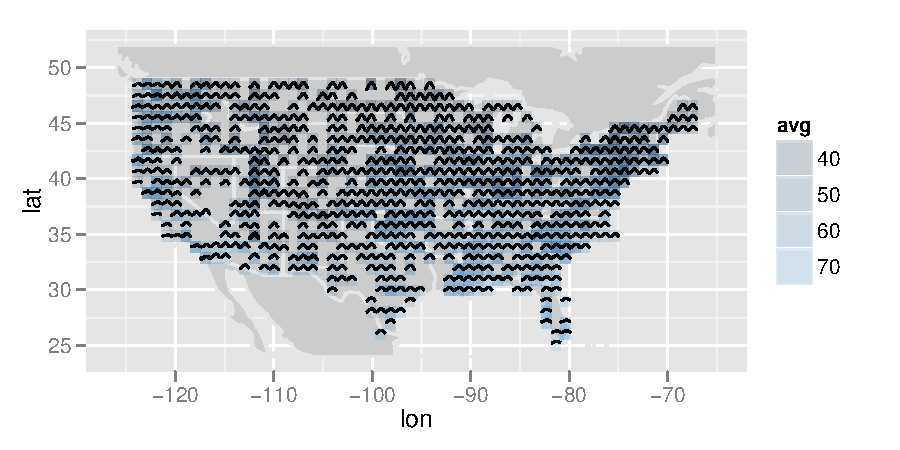
\includegraphics[width=1.05\textwidth]{figure/minimal-glyphmaps-fig-11} 

}


\end{knitrout}


\begin{knitrout}
\definecolor{shadecolor}{rgb}{0.969, 0.969, 0.969}\color{fgcolor}\begin{kframe}
\begin{flushleft}
\ttfamily\noindent
\hlfunctioncall{ggplot}\hlkeyword{(}\hlsymbol{nasa}\hlkeyword{)}{\ }\hlkeyword{+}{\ }{\ }\hlsymbol{map\usebox{\hlnormalsizeboxunderscore}nasa}{\ }\hlkeyword{+}\hspace*{\fill}\\
\hlstd{}{\ }{\ }\hlfunctioncall{glyph}\hlkeyword{(}\hlfunctioncall{geom\usebox{\hlnormalsizeboxunderscore}star}\hlkeyword{(}\hlfunctioncall{aes}\hlkeyword{(}\hlargument{r}{\ }\hlargument{=}{\ }\hlsymbol{ozone}\hlkeyword{,}{\ }\hlargument{angle}{\ }\hlargument{=}{\ }\hlsymbol{date}\hlkeyword{,}{\ }\hlargument{x}{\ }\hlargument{=}{\ }\hlnumber{0}\hlkeyword{,}{\ }\hlargument{y}{\ }\hlargument{=}{\ }\hlnumber{0}\hlkeyword{,}{\ }\hlargument{fill}{\ }\hlargument{=}{\ }\hlfunctioncall{mean}\hlkeyword{(}\hlsymbol{temperature}\hlkeyword{)}\hlkeyword{)}\hlkeyword{)}\hlkeyword{,}\hspace*{\fill}\\
\hlstd{}{\ }{\ }\hlargument{major.aes}{\ }\hlargument{=}{\ }\hlfunctioncall{aes}\hlkeyword{(}\hlsymbol{long}\hlkeyword{[}\hlnumber{1}\hlkeyword{]}\hlkeyword{,}{\ }\hlsymbol{lat}\hlkeyword{[}\hlnumber{1}\hlkeyword{]}\hlkeyword{)}\hlkeyword{,}{\ }\hlargument{glyph.by}{\ }\hlargument{=}{\ }\hlfunctioncall{c}\hlkeyword{(}\hlstring{"{}long"{}}\hlkeyword{,}{\ }\hlstring{"{}lat"{}}\hlkeyword{)}\hlkeyword{)}\mbox{}
\normalfont
\end{flushleft}
\end{kframe}

{\centering 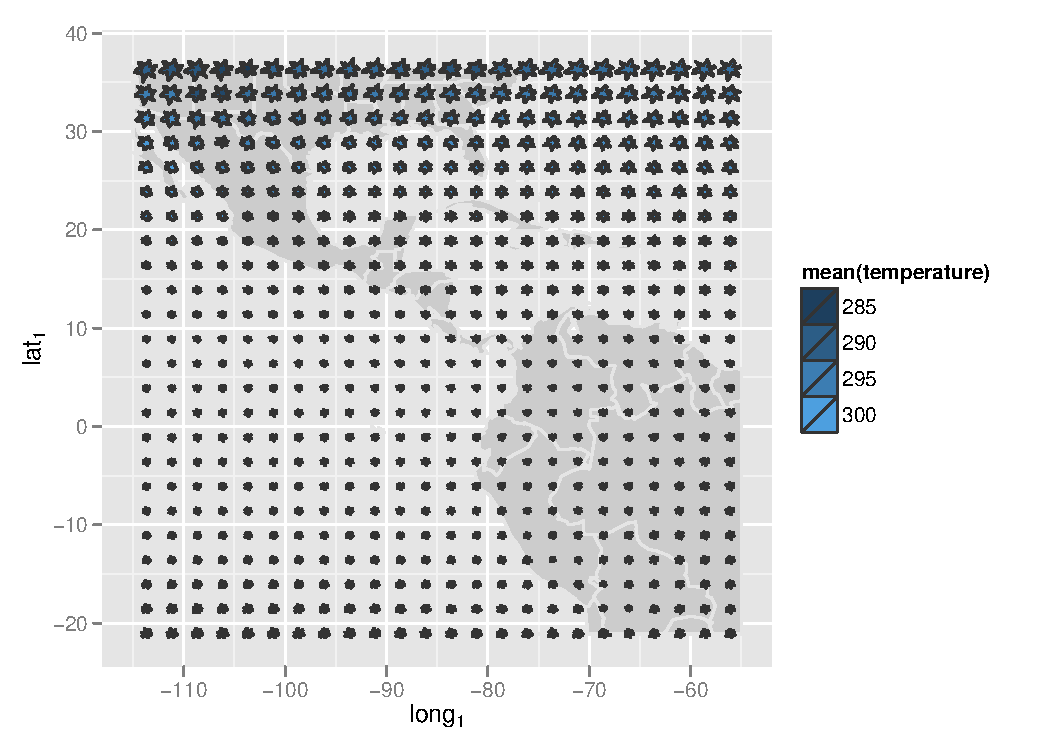
\includegraphics[width=0.8\textwidth]{figure/minimal-split-fig} 

}


\end{knitrout}


\texttt{glyphmaps} helps users create embedded graphics: plots that have subplots built into them. The package is built around three main functions: \texttt{grid}, \texttt{glyph}, and \texttt{ply$\_$aes}. This demo will demonstrate these three functions, their options, and the various uses of embedded graphics. 

\section{Glyphs}
Glyphs are geometric objects (i.e, geoms) that display information within the geom. In other words, a glyph can display information even if it is drawn by itself, without references to an external coordinate system. In reality, all geoms are a type of glyph, but the term glyph is usually reserved for complicated geoms, such as those that contain their own internal coordinate systems. The star glyphs in Figure~\ref{fig:star-glyphs} illustrate how glyphs can contain an internal (minor) coordinate system and can still be plotted in an external (major) coordinate system.

\begin{knitrout}
\definecolor{shadecolor}{rgb}{0.969, 0.969, 0.969}\color{fgcolor}\begin{figure}[]


{\centering 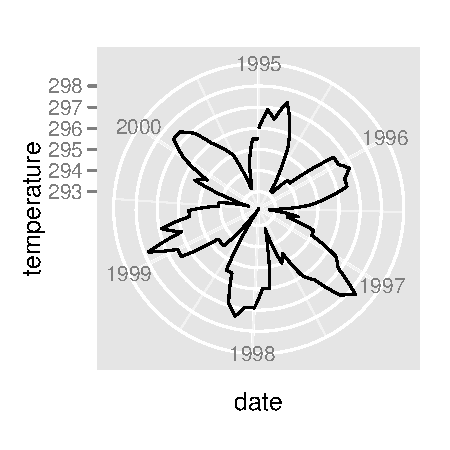
\includegraphics[width=0.49\textwidth]{figure/minimal-star-glyphs1} 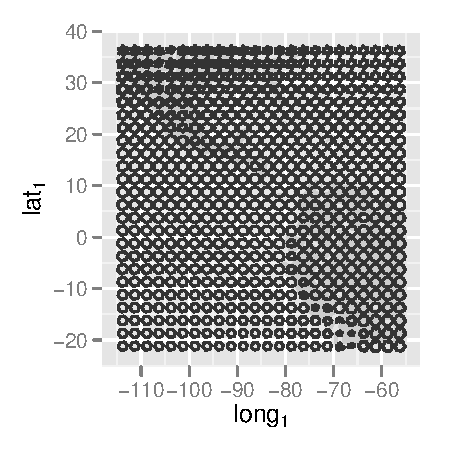
\includegraphics[width=0.49\textwidth]{figure/minimal-star-glyphs2} 

}

\caption['Individual star glyphs comprise a complete polar plot with an internal coordinate system (r = temperature and angle = date)]{'Individual star glyphs comprise a complete polar plot with an internal coordinate system (r = temperature and angle = date). Multiple star glyphs can be organized with an external coordinate sytem to reveal second order effects.'\label{fig:star-glyphs}}
\end{figure}

\end{knitrout}


Glyphs provide one connection between the grammar and graphics and embedded plots. Every glyph is an embedded plot and each embedded plot is a type of glyph. Hence, we can treat embedded plots as a type of geom. Embedded plots can also be thought of as facetting on a continuous scale. However, since embedded plots are often used with other non-facetted layers, it is easier to implement embedded plots as a type of geom.

\subsection{glyph}
\texttt{glyph} provides a general method for creating glyph geoms in \texttt{ggplot2}. \texttt{glyph} works in conjunction with \texttt{ggplot2} layer objects in the following way. Each layer specifies a type of graph through a combination of geom, stat, aesthetics, parameters, and a position adjustment. \texttt{glyph} uses this specification to build the individual glyphs (i.e, \texttt{glyph} builds glyphs that match the plot specified by the layer). \texttt{glyph} will plot a separate glyph for different subsets of the layer's data. Users specify how to split the data into subsets with the \texttt{glyph.by} argument. This argument behaves similarly to the \texttt{.variables} argument in the \texttt{plyr} package \citep{wickham2011split}. Finally, \texttt{glyph} plots each glyph on the x and y axis specified by the \texttt{major.aes} argument. These ``major axiis'' are mapped to the data just as other \texttt{ggplot2} aesthetics are mapped to the data. Hence they should be specified with the \texttt{aes} function.

To summarize, a layer can be turned into a set of glyphs with the glyph function and three arguments:
\begin{knitrout}
\definecolor{shadecolor}{rgb}{0.969, 0.969, 0.969}\color{fgcolor}\begin{kframe}
\begin{flushleft}
\ttfamily\noindent
\hlsymbol{points}{\ }\hlassignement{\usebox{\hlnormalsizeboxlessthan}-}{\ }\hlfunctioncall{geom\usebox{\hlnormalsizeboxunderscore}point}\hlkeyword{(}\hlfunctioncall{aes}\hlkeyword{(}\hlargument{x}{\ }\hlargument{=}{\ }\hlsymbol{surftemp}\hlkeyword{,}{\ }\hlargument{y}{\ }\hlargument{=}{\ }\hlsymbol{temperature}\hlkeyword{)}\hlkeyword{,}{\ }\hlargument{size}{\ }\hlargument{=}{\ }\hlnumber{1}\hlkeyword{/}\hlnumber{2}\hlkeyword{)}\hspace*{\fill}\\
\hlstd{}\hlcomment{\usebox{\hlnormalsizeboxhash}\usebox{\hlnormalsizeboxhash}{\ }A{\ }normal{\ }plot}\hspace*{\fill}\\
\hlstd{}\hlfunctioncall{ggplot}\hlkeyword{(}\hlsymbol{nasa}\hlkeyword{)}{\ }\hlkeyword{+}{\ }\hlsymbol{points}\hspace*{\fill}\\
\hlstd{}\hlcomment{\usebox{\hlnormalsizeboxhash}\usebox{\hlnormalsizeboxhash}{\ }Glyphed{\ }plot}\hspace*{\fill}\\
\hlstd{}\hlfunctioncall{ggplot}\hlkeyword{(}\hlsymbol{nasa}\hlkeyword{)}{\ }\hlkeyword{+}{\ }\hlfunctioncall{glyph}\hlkeyword{(}\hlargument{layer}{\ }\hlargument{=}{\ }\hlsymbol{points}\hlkeyword{,}{\ }\hlargument{major}{\ }\hlargument{=}{\ }\hlfunctioncall{aes}\hlkeyword{(}\hlargument{x}{\ }\hlargument{=}{\ }\hlsymbol{long}\hlkeyword{[}\hlnumber{1}\hlkeyword{]}\hlkeyword{,}{\ }\hlargument{y}{\ }\hlargument{=}{\ }\hlsymbol{lat}\hlkeyword{[}\hlnumber{1}\hlkeyword{]}\hlkeyword{)}\hlkeyword{,}\hspace*{\fill}\\
\hlstd{}{\ }{\ }{\ }{\ }\hlargument{glyph.by}{\ }\hlargument{=}{\ }\hlfunctioncall{c}\hlkeyword{(}\hlstring{"{}lat"{}}\hlkeyword{,}{\ }\hlstring{"{}long"{}}\hlkeyword{)}\hlkeyword{)}\mbox{}
\normalfont
\end{flushleft}
\end{kframe}

{\centering 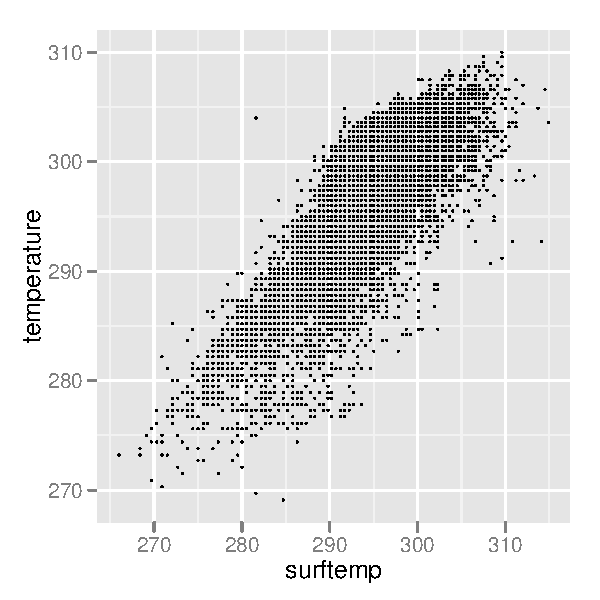
\includegraphics[width=0.49\textwidth]{figure/minimal-glyph-example1} 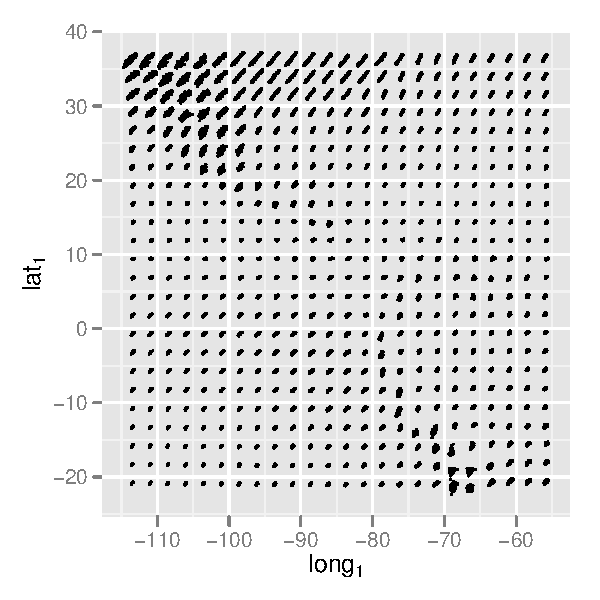
\includegraphics[width=0.49\textwidth]{figure/minimal-glyph-example2} 

}


\end{knitrout}


\texttt{glyph} gives users incredible freedom to design their own types of glyphs. Any graph that can be specified with a single layer in \texttt{ggplot2} can be turned into a glyph. \texttt{glyphmaps} also provides two new geoms that can be used to create frequently seen glyphs. These are \texttt{geom$\_$star} and \texttt{geom$\_$coxcomb}, see Figure~\ref{fig:star}. Although coxcomb glyphs don't seem much better than Venn pie-agrams (which I suppose we could also do with glyphmaps).
\begin{knitrout}
\definecolor{shadecolor}{rgb}{0.969, 0.969, 0.969}\color{fgcolor}\begin{kframe}
\begin{flushleft}
\ttfamily\noindent
\hlfunctioncall{ggplot}\hlkeyword{(}\hlsymbol{nasa}\hlkeyword{)}{\ }\hlkeyword{+}{\ }\hlfunctioncall{geom\usebox{\hlnormalsizeboxunderscore}star}\hlkeyword{(}\hlfunctioncall{aes}\hlkeyword{(}\hlargument{r}{\ }\hlargument{=}{\ }\hlsymbol{ozone}\hlkeyword{,}{\ }\hlargument{angle}{\ }\hlargument{=}{\ }\hlsymbol{date}\hlkeyword{,}{\ }\hlargument{x}{\ }\hlargument{=}{\ }\hlnumber{0}\hlkeyword{,}{\ }\hlargument{y}{\ }\hlargument{=}{\ }\hlnumber{0}\hlkeyword{,}\hspace*{\fill}\\
\hlstd{}{\ }{\ }{\ }{\ }\hlargument{fill}{\ }\hlargument{=}{\ }\hlfunctioncall{mean}\hlkeyword{(}\hlsymbol{ozone}\hlkeyword{)}\hlkeyword{)}\hlkeyword{,}{\ }\hlargument{alpha}{\ }\hlargument{=}{\ }\hlnumber{0.5}\hlkeyword{)}\hspace*{\fill}\\
\hlstd{}\hlfunctioncall{ggplot}\hlkeyword{(}\hlsymbol{seasons}\hlkeyword{)}{\ }\hlkeyword{+}{\ }\hlfunctioncall{geom\usebox{\hlnormalsizeboxunderscore}coxcomb}\hlkeyword{(}\hlfunctioncall{aes}\hlkeyword{(}\hlargument{angle}{\ }\hlargument{=}{\ }\hlsymbol{state}\hlkeyword{,}{\ }\hlargument{fill}{\ }\hlargument{=}{\ }\hlsymbol{lat}\hlkeyword{)}\hlkeyword{)}\mbox{}
\normalfont
\end{flushleft}
\end{kframe}

{\centering 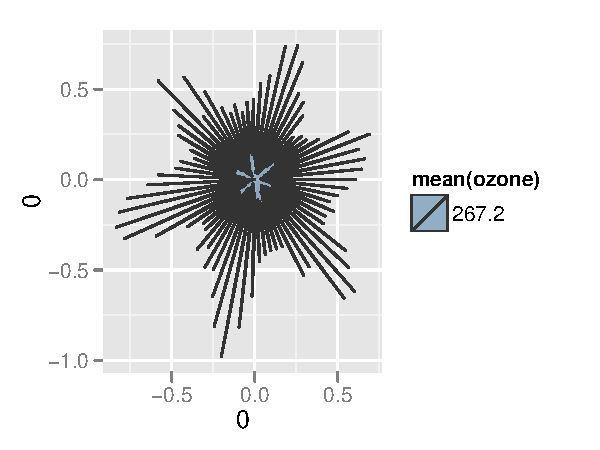
\includegraphics[width=0.49\textwidth]{figure/minimal-star1} 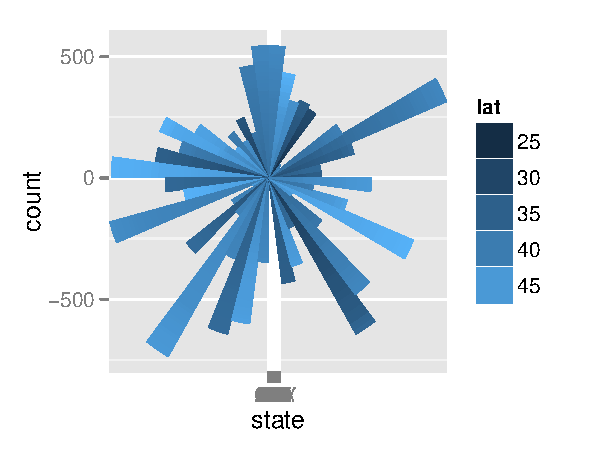
\includegraphics[width=0.49\textwidth]{figure/minimal-star2} 

}


\end{knitrout}


\texttt{glyph} also has a variety of optional arguments that allow users to customize glyph plots. These allow the user to control the dimensions of each glyph, to control the scale within each glyph, to add reference objects to each glyph, and to merge glyphs that overlap into a single glyph.

\subsubsection{width, height}
The \texttt{width} and \texttt{height} arguments of \texttt{glyph} control the width and height of each glyph in the plot.
\begin{knitrout}
\definecolor{shadecolor}{rgb}{0.969, 0.969, 0.969}\color{fgcolor}\begin{kframe}
\begin{flushleft}
\ttfamily\noindent
\hlfunctioncall{ggplot}\hlkeyword{(}\hlsymbol{mpg}\hlkeyword{)}{\ }\hlkeyword{+}{\ }\hlfunctioncall{glyph}\hlkeyword{(}\hlfunctioncall{geom\usebox{\hlnormalsizeboxunderscore}bar}\hlkeyword{(}\hlfunctioncall{aes}\hlkeyword{(}\hlargument{x}{\ }\hlargument{=}{\ }\hlsymbol{trans}\hlkeyword{,}{\ }\hlargument{fill}{\ }\hlargument{=}{\ }\hlsymbol{year}\hlkeyword{)}\hlkeyword{)}\hlkeyword{,}\hspace*{\fill}\\
\hlstd{}{\ }{\ }\hlfunctioncall{aes}\hlkeyword{(}\hlargument{x}{\ }\hlargument{=}{\ }\hlfunctioncall{mean}\hlkeyword{(}\hlsymbol{displ}\hlkeyword{)}\hlkeyword{,}{\ }\hlargument{y}{\ }\hlargument{=}{\ }\hlfunctioncall{mean}\hlkeyword{(}\hlsymbol{cty}\hlkeyword{)}\hlkeyword{)}\hlkeyword{,}{\ }\hlfunctioncall{c}\hlkeyword{(}\hlstring{"{}year"{}}\hlkeyword{)}\hlkeyword{)}\hspace*{\fill}\\
\hlstd{}\hlfunctioncall{ggplot}\hlkeyword{(}\hlsymbol{mpg}\hlkeyword{)}{\ }\hlkeyword{+}{\ }\hlfunctioncall{glyph}\hlkeyword{(}\hlfunctioncall{geom\usebox{\hlnormalsizeboxunderscore}bar}\hlkeyword{(}\hlfunctioncall{aes}\hlkeyword{(}\hlargument{x}{\ }\hlargument{=}{\ }\hlsymbol{trans}\hlkeyword{,}{\ }\hlargument{fill}{\ }\hlargument{=}{\ }\hlsymbol{year}\hlkeyword{)}\hlkeyword{)}\hlkeyword{,}\hspace*{\fill}\\
\hlstd{}{\ }{\ }\hlfunctioncall{aes}\hlkeyword{(}\hlargument{x}{\ }\hlargument{=}{\ }\hlfunctioncall{mean}\hlkeyword{(}\hlsymbol{displ}\hlkeyword{)}\hlkeyword{,}{\ }\hlargument{y}{\ }\hlargument{=}{\ }\hlfunctioncall{mean}\hlkeyword{(}\hlsymbol{cty}\hlkeyword{)}\hlkeyword{)}\hlkeyword{,}{\ }\hlfunctioncall{c}\hlkeyword{(}\hlstring{"{}year"{}}\hlkeyword{)}\hlkeyword{,}\hspace*{\fill}\\
\hlstd{}{\ }{\ }\hlargument{width}{\ }\hlargument{=}{\ }\hlnumber{1}\hlkeyword{/}\hlnumber{4}\hlkeyword{,}{\ }\hlargument{height}{\ }\hlargument{=}{\ }\hlnumber{1}\hlkeyword{/}\hlnumber{4}\hlkeyword{)}\mbox{}
\normalfont
\end{flushleft}
\end{kframe}

{\centering 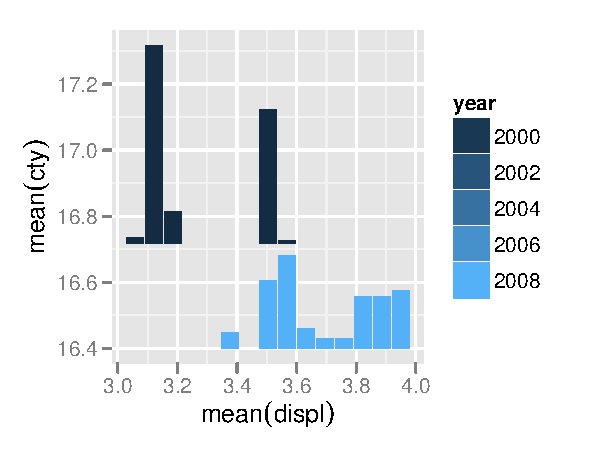
\includegraphics[width=0.49\textwidth]{figure/minimal-dims1} 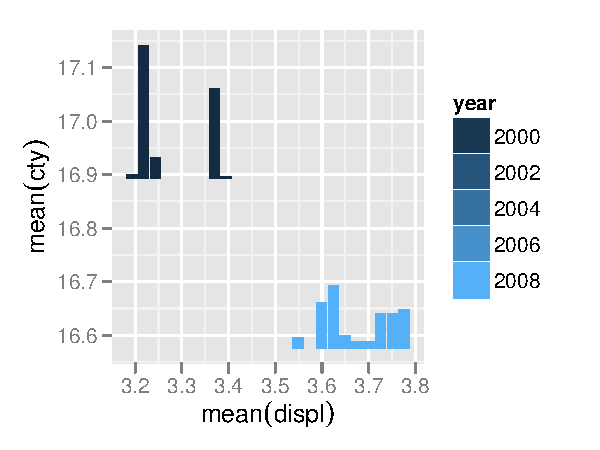
\includegraphics[width=0.49\textwidth]{figure/minimal-dims2} 

}


\end{knitrout}


\subsubsection{x$\_$scale, y$\_$scale}
The \texttt{x$\_$scale} and \texttt{y$\_$scale} arguments of \texttt{glyph} control the scaling within each glyph. As with facets, glyphs share the same scaling by default. The x and y scales can also be set to `free'.
\begin{knitrout}
\definecolor{shadecolor}{rgb}{0.969, 0.969, 0.969}\color{fgcolor}\begin{kframe}
\begin{flushleft}
\ttfamily\noindent
\hlcomment{\usebox{\hlnormalsizeboxhash}\usebox{\hlnormalsizeboxhash}{\ }glyphs{\ }share{\ }y{\ }scale}\hspace*{\fill}\\
\hlstd{}\hlfunctioncall{ggplot}\hlkeyword{(}\hlsymbol{mpg}\hlkeyword{)}{\ }\hlkeyword{+}{\ }\hlfunctioncall{glyph}\hlkeyword{(}\hlfunctioncall{geom\usebox{\hlnormalsizeboxunderscore}bar}\hlkeyword{(}\hlfunctioncall{aes}\hlkeyword{(}\hlargument{x}{\ }\hlargument{=}{\ }\hlsymbol{trans}\hlkeyword{,}{\ }\hlargument{fill}{\ }\hlargument{=}{\ }\hlsymbol{year}\hlkeyword{)}\hlkeyword{)}\hlkeyword{,}\hspace*{\fill}\\
\hlstd{}{\ }{\ }\hlfunctioncall{aes}\hlkeyword{(}\hlargument{x}{\ }\hlargument{=}{\ }\hlfunctioncall{mean}\hlkeyword{(}\hlsymbol{displ}\hlkeyword{)}\hlkeyword{,}{\ }\hlargument{y}{\ }\hlargument{=}{\ }\hlfunctioncall{mean}\hlkeyword{(}\hlsymbol{cty}\hlkeyword{)}\hlkeyword{)}\hlkeyword{,}{\ }\hlfunctioncall{c}\hlkeyword{(}\hlstring{"{}year"{}}\hlkeyword{)}\hlkeyword{,}\hspace*{\fill}\\
\hlstd{}{\ }{\ }\hlargument{width}{\ }\hlargument{=}{\ }\hlnumber{1}\hlkeyword{/}\hlnumber{4}\hlkeyword{,}{\ }\hlargument{height}{\ }\hlargument{=}{\ }\hlnumber{1}\hlkeyword{/}\hlnumber{4}\hlkeyword{)}\hspace*{\fill}\\
\hlstd{}\hlcomment{\usebox{\hlnormalsizeboxhash}\usebox{\hlnormalsizeboxhash}{\ }independent{\ }y{\ }scales}\hspace*{\fill}\\
\hlstd{}\hlfunctioncall{ggplot}\hlkeyword{(}\hlsymbol{mpg}\hlkeyword{)}{\ }\hlkeyword{+}{\ }\hlfunctioncall{glyph}\hlkeyword{(}\hlfunctioncall{geom\usebox{\hlnormalsizeboxunderscore}bar}\hlkeyword{(}\hlfunctioncall{aes}\hlkeyword{(}\hlargument{x}{\ }\hlargument{=}{\ }\hlsymbol{trans}\hlkeyword{,}{\ }\hlargument{fill}{\ }\hlargument{=}{\ }\hlsymbol{year}\hlkeyword{)}\hlkeyword{)}\hlkeyword{,}\hspace*{\fill}\\
\hlstd{}{\ }{\ }\hlfunctioncall{aes}\hlkeyword{(}\hlargument{x}{\ }\hlargument{=}{\ }\hlfunctioncall{mean}\hlkeyword{(}\hlsymbol{displ}\hlkeyword{)}\hlkeyword{,}{\ }\hlargument{y}{\ }\hlargument{=}{\ }\hlfunctioncall{mean}\hlkeyword{(}\hlsymbol{cty}\hlkeyword{)}\hlkeyword{)}\hlkeyword{,}{\ }\hlfunctioncall{c}\hlkeyword{(}\hlstring{"{}year"{}}\hlkeyword{)}\hlkeyword{,}\hspace*{\fill}\\
\hlstd{}{\ }{\ }\hlargument{width}{\ }\hlargument{=}{\ }\hlnumber{1}\hlkeyword{/}\hlnumber{4}\hlkeyword{,}{\ }\hlargument{height}{\ }\hlargument{=}{\ }\hlnumber{1}\hlkeyword{/}\hlnumber{4}\hlkeyword{,}{\ }\hlargument{y\usebox{\hlnormalsizeboxunderscore}scale}{\ }\hlargument{=}{\ }\hlsymbol{free}\hlkeyword{)}\mbox{}
\normalfont
\end{flushleft}
\end{kframe}

{\centering 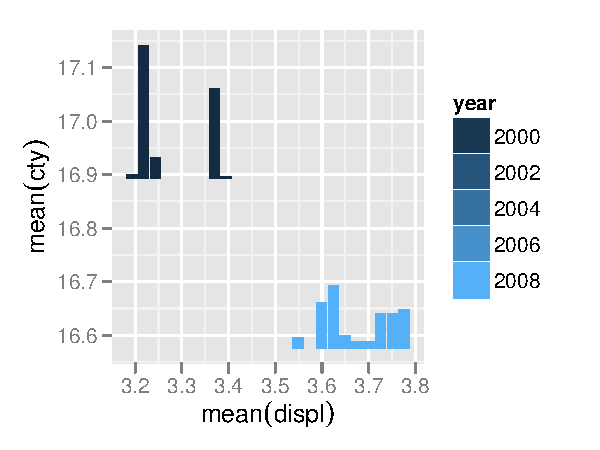
\includegraphics[width=0.49\textwidth]{figure/minimal-scales1} 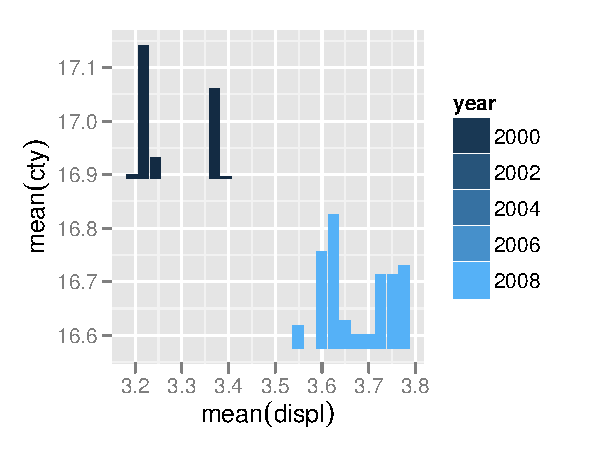
\includegraphics[width=0.49\textwidth]{figure/minimal-scales2} 

}


\end{knitrout}


\subsubsection{reference objects}
Users can set the \texttt{reference} argument to include reference objects with each glyph. These objects provide a frame of reference which facilitates comparing between glyphs. The \texttt{reference} argument should be set to one of \texttt{ref$\_$box}, \texttt{ref$\_$hline}, \texttt{ref$\_$vline}, \texttt{ref$\_$points}, or \texttt{NULL}. Each of these functions creates a different type of reference object, see Figure~\ref{fig:refs}. Each also accepts a mapping and parameters to customize the appearance of the reference objects.
\begin{knitrout}
\definecolor{shadecolor}{rgb}{0.969, 0.969, 0.969}\color{fgcolor}\begin{kframe}
\begin{flushleft}
\ttfamily\noindent
\hlcomment{\usebox{\hlnormalsizeboxhash}{\ }boxes}\hspace*{\fill}\\
\hlstd{}\hlfunctioncall{ggplot}\hlkeyword{(}\hlsymbol{test.data}\hlkeyword{)}{\ }\hlkeyword{+}{\ }\hlfunctioncall{glyph}\hlkeyword{(}\hlfunctioncall{geom\usebox{\hlnormalsizeboxunderscore}point}\hlkeyword{(}\hlfunctioncall{aes}\hlkeyword{(}\hlsymbol{Fertility}\hlkeyword{,}{\ }\hlsymbol{Agriculture}\hlkeyword{,}\hspace*{\fill}\\
\hlstd{}{\ }{\ }\hlargument{color}{\ }\hlargument{=}{\ }\hlfunctioncall{rank}\hlkeyword{(}\hlsymbol{Catholic}\hlkeyword{)}\hlkeyword{)}\hlkeyword{)}\hlkeyword{,}{\ }\hlargument{glyph.by}{\ }\hlargument{=}{\ }\hlfunctioncall{c}\hlkeyword{(}\hlstring{"{}lat"{}}\hlkeyword{,}{\ }\hlstring{"{}long"{}}\hlkeyword{)}\hlkeyword{,}\hspace*{\fill}\\
\hlstd{}{\ }{\ }\hlargument{major}{\ }\hlargument{=}{\ }\hlfunctioncall{aes}\hlkeyword{(}\hlfunctioncall{mean}\hlkeyword{(}\hlsymbol{Fertility}\hlkeyword{)}\hlkeyword{,}{\ }\hlfunctioncall{mean}\hlkeyword{(}\hlsymbol{Education}\hlkeyword{)}\hlkeyword{)}\hlkeyword{,}{\ }\hlargument{ref}{\ }\hlargument{=}{\ }\hlfunctioncall{ref\usebox{\hlnormalsizeboxunderscore}box}\hlkeyword{(}\hlfunctioncall{aes}\hlkeyword{(}\hlargument{fill}{\ }\hlargument{=}\hspace*{\fill}\\
\hlstd{}{\ }{\ }\hlfunctioncall{mean}\hlkeyword{(}\hlsymbol{Catholic}\hlkeyword{)}\hlkeyword{)}\hlkeyword{)}\hlkeyword{)}\hspace*{\fill}\\
\hlstd{}\hspace*{\fill}\\
\hlstd{}\hlcomment{\usebox{\hlnormalsizeboxhash}{\ }hlines}\hspace*{\fill}\\
\hlstd{}\hlfunctioncall{ggplot}\hlkeyword{(}\hlsymbol{test.data}\hlkeyword{)}{\ }\hlkeyword{+}{\ }\hlfunctioncall{glyph}\hlkeyword{(}\hlfunctioncall{geom\usebox{\hlnormalsizeboxunderscore}point}\hlkeyword{(}\hlfunctioncall{aes}\hlkeyword{(}\hlsymbol{Fertility}\hlkeyword{,}{\ }\hlsymbol{Agriculture}\hlkeyword{,}\hspace*{\fill}\\
\hlstd{}{\ }{\ }\hlargument{color}{\ }\hlargument{=}{\ }\hlfunctioncall{rank}\hlkeyword{(}\hlsymbol{Catholic}\hlkeyword{)}\hlkeyword{)}\hlkeyword{)}\hlkeyword{,}{\ }\hlargument{glyph.by}{\ }\hlargument{=}{\ }\hlfunctioncall{c}\hlkeyword{(}\hlstring{"{}lat"{}}\hlkeyword{,}{\ }\hlstring{"{}long"{}}\hlkeyword{)}\hlkeyword{,}\hspace*{\fill}\\
\hlstd{}{\ }{\ }\hlargument{major}{\ }\hlargument{=}{\ }\hlfunctioncall{aes}\hlkeyword{(}\hlfunctioncall{mean}\hlkeyword{(}\hlsymbol{Fertility}\hlkeyword{)}\hlkeyword{,}{\ }\hlfunctioncall{mean}\hlkeyword{(}\hlsymbol{Education}\hlkeyword{)}\hlkeyword{)}\hlkeyword{,}{\ }\hlargument{ref}{\ }\hlargument{=}{\ }\hlfunctioncall{ref\usebox{\hlnormalsizeboxunderscore}hline}\hlkeyword{(}\hlfunctioncall{aes}\hlkeyword{(}\hlargument{fill}{\ }\hlargument{=}\hspace*{\fill}\\
\hlstd{}{\ }{\ }\hlfunctioncall{mean}\hlkeyword{(}\hlsymbol{Catholic}\hlkeyword{)}\hlkeyword{)}\hlkeyword{)}\hlkeyword{)}\hspace*{\fill}\\
\hlstd{}\hspace*{\fill}\\
\hlstd{}\hlcomment{\usebox{\hlnormalsizeboxhash}{\ }vlines}\hspace*{\fill}\\
\hlstd{}\hlfunctioncall{ggplot}\hlkeyword{(}\hlsymbol{test.data}\hlkeyword{)}{\ }\hlkeyword{+}{\ }\hlfunctioncall{glyph}\hlkeyword{(}\hlfunctioncall{geom\usebox{\hlnormalsizeboxunderscore}point}\hlkeyword{(}\hlfunctioncall{aes}\hlkeyword{(}\hlsymbol{Fertility}\hlkeyword{,}{\ }\hlsymbol{Agriculture}\hlkeyword{,}\hspace*{\fill}\\
\hlstd{}{\ }{\ }\hlargument{color}{\ }\hlargument{=}{\ }\hlfunctioncall{rank}\hlkeyword{(}\hlsymbol{Catholic}\hlkeyword{)}\hlkeyword{)}\hlkeyword{)}\hlkeyword{,}{\ }\hlargument{glyph.by}{\ }\hlargument{=}{\ }\hlfunctioncall{c}\hlkeyword{(}\hlstring{"{}lat"{}}\hlkeyword{,}{\ }\hlstring{"{}long"{}}\hlkeyword{)}\hlkeyword{,}\hspace*{\fill}\\
\hlstd{}{\ }{\ }\hlargument{major}{\ }\hlargument{=}{\ }\hlfunctioncall{aes}\hlkeyword{(}\hlfunctioncall{mean}\hlkeyword{(}\hlsymbol{Fertility}\hlkeyword{)}\hlkeyword{,}{\ }\hlfunctioncall{mean}\hlkeyword{(}\hlsymbol{Education}\hlkeyword{)}\hlkeyword{)}\hlkeyword{,}{\ }\hlargument{ref}{\ }\hlargument{=}{\ }\hlfunctioncall{ref\usebox{\hlnormalsizeboxunderscore}vline}\hlkeyword{(}\hlfunctioncall{aes}\hlkeyword{(}\hlargument{fill}{\ }\hlargument{=}\hspace*{\fill}\\
\hlstd{}{\ }{\ }\hlfunctioncall{mean}\hlkeyword{(}\hlsymbol{Catholic}\hlkeyword{)}\hlkeyword{)}\hlkeyword{)}\hlkeyword{)}\hspace*{\fill}\\
\hlstd{}\hspace*{\fill}\\
\hlstd{}\hlcomment{\usebox{\hlnormalsizeboxhash}{\ }points}\hspace*{\fill}\\
\hlstd{}\hlfunctioncall{ggplot}\hlkeyword{(}\hlsymbol{mpg}\hlkeyword{)}{\ }\hlkeyword{+}{\ }\hlfunctioncall{glyph}\hlkeyword{(}\hlfunctioncall{geom\usebox{\hlnormalsizeboxunderscore}bar}\hlkeyword{(}\hlfunctioncall{aes}\hlkeyword{(}\hlargument{x}{\ }\hlargument{=}{\ }\hlsymbol{trans}\hlkeyword{,}{\ }\hlargument{fill}{\ }\hlargument{=}{\ }\hlsymbol{year}\hlkeyword{)}\hlkeyword{)}\hlkeyword{,}\hspace*{\fill}\\
\hlstd{}{\ }{\ }\hlfunctioncall{aes}\hlkeyword{(}\hlargument{x}{\ }\hlargument{=}{\ }\hlfunctioncall{mean}\hlkeyword{(}\hlsymbol{displ}\hlkeyword{)}\hlkeyword{,}{\ }\hlargument{y}{\ }\hlargument{=}{\ }\hlfunctioncall{mean}\hlkeyword{(}\hlsymbol{cty}\hlkeyword{)}\hlkeyword{)}\hlkeyword{,}{\ }\hlfunctioncall{c}\hlkeyword{(}\hlstring{"{}year"{}}\hlkeyword{)}\hlkeyword{,}{\ }\hlargument{y\usebox{\hlnormalsizeboxunderscore}scale}{\ }\hlargument{=}{\ }\hlsymbol{free}\hlkeyword{,}\hspace*{\fill}\\
\hlstd{}{\ }{\ }\hlargument{width}{\ }\hlargument{=}{\ }\hlnumber{1}\hlkeyword{/}\hlnumber{3}\hlkeyword{,}{\ }\hlargument{height}{\ }\hlargument{=}{\ }\hlnumber{1}\hlkeyword{/}\hlnumber{3}\hlkeyword{,}{\ }\hlargument{reference}{\ }\hlargument{=}{\ }\hlfunctioncall{ref\usebox{\hlnormalsizeboxunderscore}points}\hlkeyword{(}\hlfunctioncall{aes}\hlkeyword{(}\hlargument{fill}{\ }\hlargument{=}{\ }\hlfunctioncall{mean}\hlkeyword{(}\hlsymbol{hwy}\hlkeyword{)}\hlkeyword{)}\hlkeyword{)}\hlkeyword{)}\mbox{}
\normalfont
\end{flushleft}
\end{kframe}

{\centering 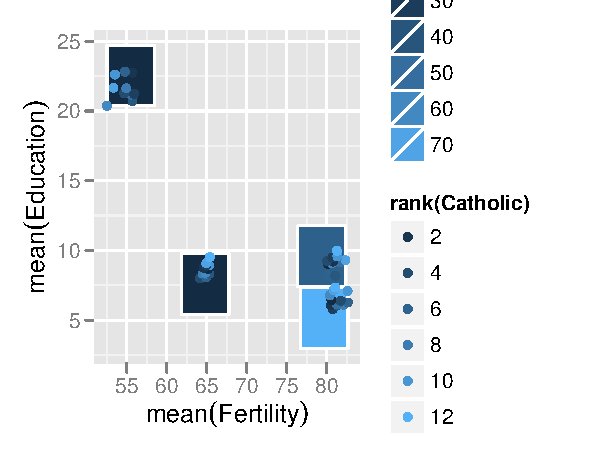
\includegraphics[width=0.49\textwidth]{figure/minimal-refs1} 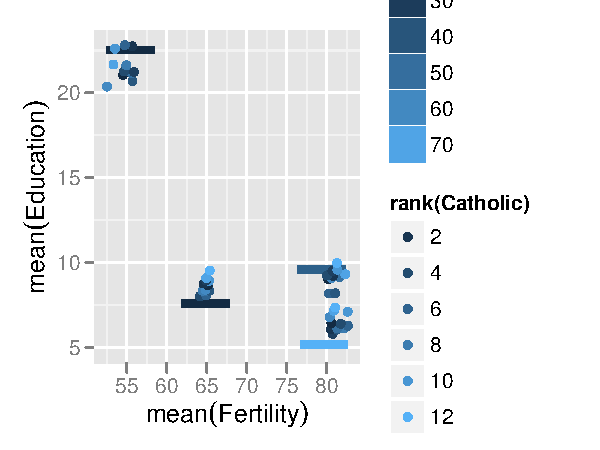
\includegraphics[width=0.49\textwidth]{figure/minimal-refs2} 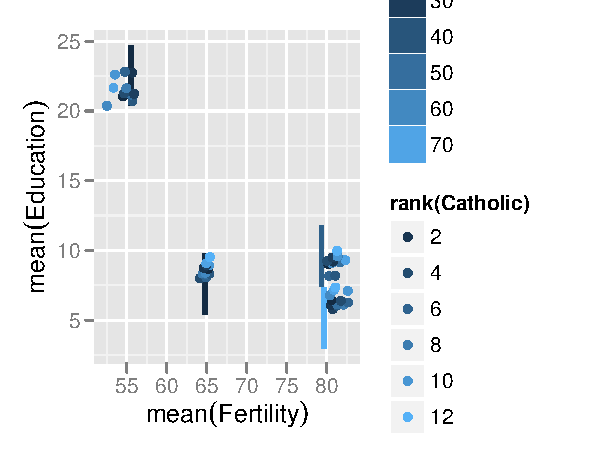
\includegraphics[width=0.49\textwidth]{figure/minimal-refs3} 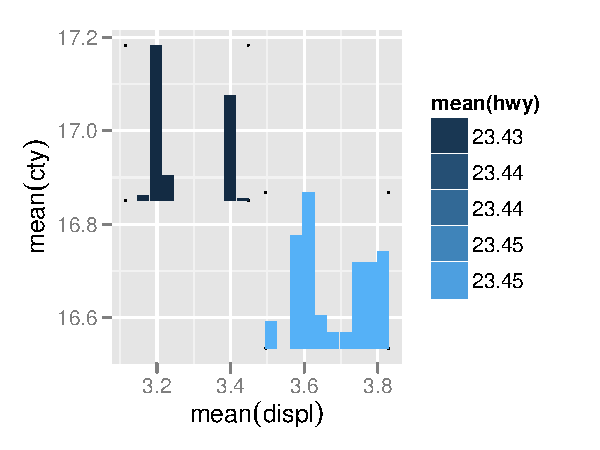
\includegraphics[width=0.49\textwidth]{figure/minimal-refs4} 

}


\end{knitrout}


\subsection{merge overlaps}
Often two or more glyphs will overlap each other when plotted. It is possible to combine such overlapping glyphs into a single glyph by setting the \texttt{merge.overlaps} argument to \texttt{TRUE}. \texttt{glyphmaps} will then screen the glyph output for sets of overlapping graphs. Each set will be combined into one glyph and plotted at the at the average location of the combined glyphs, see Figure~\ref{fig:overlaps}.
Caution should be used when setting \texttt{merge.overlaps} to \texttt{TRUE}. Merge overlaps currently works \emph{exactly} as described, which means that for very dense graphs, \texttt{merge.overlaps} is likely to thin out the plot a bit more than the user expects.
\begin{knitrout}
\definecolor{shadecolor}{rgb}{0.969, 0.969, 0.969}\color{fgcolor}\begin{kframe}
\begin{flushleft}
\ttfamily\noindent
\hlcomment{\usebox{\hlnormalsizeboxhash}\usebox{\hlnormalsizeboxhash}{\ }no{\ }merging{\ }}\hspace*{\fill}\\
\hlstd{}\hlfunctioncall{ggplot}\hlkeyword{(}\hlsymbol{test.data}\hlkeyword{)}{\ }\hlkeyword{+}{\ }\hlfunctioncall{glyph}\hlkeyword{(}\hlfunctioncall{geom\usebox{\hlnormalsizeboxunderscore}point}\hlkeyword{(}\hlfunctioncall{aes}\hlkeyword{(}\hlsymbol{Fertility}\hlkeyword{,}{\ }\hlsymbol{Agriculture}\hlkeyword{,}\hspace*{\fill}\\
\hlstd{}{\ }{\ }\hlargument{color}{\ }\hlargument{=}{\ }\hlfunctioncall{rank}\hlkeyword{(}\hlsymbol{Catholic}\hlkeyword{)}\hlkeyword{)}\hlkeyword{,}{\ }\hlargument{size}{\ }\hlargument{=}{\ }\hlnumber{3}\hlkeyword{)}\hlkeyword{,}{\ }\hlargument{glyph.by}{\ }\hlargument{=}{\ }\hlfunctioncall{c}\hlkeyword{(}\hlstring{"{}lat"{}}\hlkeyword{,}{\ }\hlstring{"{}long"{}}\hlkeyword{)}\hlkeyword{,}\hspace*{\fill}\\
\hlstd{}{\ }{\ }\hlargument{major}{\ }\hlargument{=}{\ }\hlfunctioncall{aes}\hlkeyword{(}\hlfunctioncall{mean}\hlkeyword{(}\hlsymbol{Fertility}\hlkeyword{)}\hlkeyword{,}{\ }\hlfunctioncall{mean}\hlkeyword{(}\hlsymbol{Education}\hlkeyword{)}\hlkeyword{)}\hlkeyword{,}{\ }\hlargument{ref}{\ }\hlargument{=}{\ }\hlfunctioncall{ref\usebox{\hlnormalsizeboxunderscore}box}\hlkeyword{(}\hlfunctioncall{aes}\hlkeyword{(}\hlargument{fill}{\ }\hlargument{=}\hspace*{\fill}\\
\hlstd{}{\ }{\ }\hlfunctioncall{mean}\hlkeyword{(}\hlsymbol{Catholic}\hlkeyword{)}\hlkeyword{)}\hlkeyword{)}\hlkeyword{,}{\ }\hlargument{width}{\ }\hlargument{=}{\ }\hlfunctioncall{rel}\hlkeyword{(}\hlnumber{1}\hlkeyword{)}\hlkeyword{,}{\ }\hlargument{height}{\ }\hlargument{=}{\ }\hlfunctioncall{rel}\hlkeyword{(}\hlnumber{1}\hlkeyword{)}\hlkeyword{)}\hspace*{\fill}\\
\hlstd{}\hlcomment{\usebox{\hlnormalsizeboxhash}\usebox{\hlnormalsizeboxhash}{\ }merging}\hspace*{\fill}\\
\hlstd{}\hlfunctioncall{ggplot}\hlkeyword{(}\hlsymbol{test.data}\hlkeyword{)}{\ }\hlkeyword{+}{\ }\hlfunctioncall{glyph}\hlkeyword{(}\hlfunctioncall{geom\usebox{\hlnormalsizeboxunderscore}point}\hlkeyword{(}\hlfunctioncall{aes}\hlkeyword{(}\hlsymbol{Fertility}\hlkeyword{,}{\ }\hlsymbol{Agriculture}\hlkeyword{,}\hspace*{\fill}\\
\hlstd{}{\ }{\ }\hlargument{color}{\ }\hlargument{=}{\ }\hlfunctioncall{rank}\hlkeyword{(}\hlsymbol{Catholic}\hlkeyword{)}\hlkeyword{)}\hlkeyword{,}{\ }\hlargument{size}{\ }\hlargument{=}{\ }\hlnumber{3}\hlkeyword{)}\hlkeyword{,}{\ }\hlargument{glyph.by}{\ }\hlargument{=}{\ }\hlfunctioncall{c}\hlkeyword{(}\hlstring{"{}lat"{}}\hlkeyword{,}{\ }\hlstring{"{}long"{}}\hlkeyword{)}\hlkeyword{,}\hspace*{\fill}\\
\hlstd{}{\ }{\ }\hlargument{major}{\ }\hlargument{=}{\ }\hlfunctioncall{aes}\hlkeyword{(}\hlfunctioncall{mean}\hlkeyword{(}\hlsymbol{Fertility}\hlkeyword{)}\hlkeyword{,}{\ }\hlfunctioncall{mean}\hlkeyword{(}\hlsymbol{Education}\hlkeyword{)}\hlkeyword{)}\hlkeyword{,}{\ }\hlargument{ref}{\ }\hlargument{=}{\ }\hlfunctioncall{ref\usebox{\hlnormalsizeboxunderscore}box}\hlkeyword{(}\hlfunctioncall{aes}\hlkeyword{(}\hlargument{fill}{\ }\hlargument{=}\hspace*{\fill}\\
\hlstd{}{\ }{\ }\hlfunctioncall{mean}\hlkeyword{(}\hlsymbol{Catholic}\hlkeyword{)}\hlkeyword{)}\hlkeyword{)}\hlkeyword{,}{\ }\hlargument{merge}{\ }\hlargument{=}{\ }\hlnumber{TRUE}\hlkeyword{,}{\ }\hlargument{width}{\ }\hlargument{=}{\ }\hlfunctioncall{rel}\hlkeyword{(}\hlnumber{1}\hlkeyword{)}\hlkeyword{,}{\ }\hlargument{height}{\ }\hlargument{=}{\ }\hlfunctioncall{rel}\hlkeyword{(}\hlnumber{1}\hlkeyword{)}\hlkeyword{)}\hspace*{\fill}\\
\hlstd{}\hspace*{\fill}\\
\hlstd{}\hlcomment{\usebox{\hlnormalsizeboxhash}\usebox{\hlnormalsizeboxhash}{\ }compare{\ }with{\ }dense{\ }situations}\hspace*{\fill}\\
\hlstd{}\hlfunctioncall{ggplot}\hlkeyword{(}\hlsymbol{seasons}\hlkeyword{)}{\ }\hlkeyword{+}{\ }\hlsymbol{map\usebox{\hlnormalsizeboxunderscore}us}{\ }\hlkeyword{+}\hspace*{\fill}\\
\hlstd{}{\ }{\ }\hlfunctioncall{glyph}\hlkeyword{(}\hlfunctioncall{geom\usebox{\hlnormalsizeboxunderscore}line}\hlkeyword{(}\hlfunctioncall{aes}\hlkeyword{(}\hlargument{x}{\ }\hlargument{=}{\ }\hlsymbol{time}\hlkeyword{,}{\ }\hlargument{y}{\ }\hlargument{=}{\ }\hlsymbol{pred}\hlkeyword{)}\hlkeyword{)}\hlkeyword{,}\hspace*{\fill}\\
\hlstd{}{\ }{\ }{\ }{\ }\hlfunctioncall{aes}\hlkeyword{(}\hlsymbol{lon}\hlkeyword{[}\hlnumber{1}\hlkeyword{]}\hlkeyword{,}{\ }\hlsymbol{lat}\hlkeyword{[}\hlnumber{1}\hlkeyword{]}\hlkeyword{)}\hlkeyword{,}{\ }\hlfunctioncall{c}\hlkeyword{(}\hlstring{"{}stn"{}}\hlkeyword{)}\hlkeyword{,}{\ }\hlargument{height}{\ }\hlargument{=}{\ }\hlnumber{1}\hlkeyword{,}{\ }\hlargument{width}{\ }\hlargument{=}{\ }\hlnumber{1.5}\hlkeyword{,}\hspace*{\fill}\\
\hlstd{}{\ }{\ }{\ }{\ }{\ }{\ }{\ }\hlargument{ref}{\ }\hlargument{=}{\ }\hlfunctioncall{ref\usebox{\hlnormalsizeboxunderscore}box}\hlkeyword{(}\hlfunctioncall{aes}\hlkeyword{(}\hlargument{fill}{\ }\hlargument{=}{\ }\hlsymbol{avg}\hlkeyword{)}\hlkeyword{,}{\ }\hlargument{color}{\ }\hlargument{=}{\ }\hlnumber{NA}\hlkeyword{)}\hlkeyword{)}\hspace*{\fill}\\
\hlstd{}\hlcomment{\usebox{\hlnormalsizeboxhash}\usebox{\hlnormalsizeboxhash}{\ }vs}\hspace*{\fill}\\
\hlstd{}\hlfunctioncall{ggplot}\hlkeyword{(}\hlsymbol{seasons}\hlkeyword{)}{\ }\hlkeyword{+}{\ }\hlsymbol{map\usebox{\hlnormalsizeboxunderscore}us}{\ }\hlkeyword{+}\hspace*{\fill}\\
\hlstd{}{\ }{\ }\hlfunctioncall{glyph}\hlkeyword{(}\hlfunctioncall{geom\usebox{\hlnormalsizeboxunderscore}line}\hlkeyword{(}\hlfunctioncall{aes}\hlkeyword{(}\hlargument{x}{\ }\hlargument{=}{\ }\hlsymbol{time}\hlkeyword{,}{\ }\hlargument{y}{\ }\hlargument{=}{\ }\hlsymbol{pred}\hlkeyword{)}\hlkeyword{)}\hlkeyword{,}\hspace*{\fill}\\
\hlstd{}{\ }{\ }{\ }{\ }\hlfunctioncall{aes}\hlkeyword{(}\hlsymbol{lon}\hlkeyword{[}\hlnumber{1}\hlkeyword{]}\hlkeyword{,}{\ }\hlsymbol{lat}\hlkeyword{[}\hlnumber{1}\hlkeyword{]}\hlkeyword{)}\hlkeyword{,}{\ }\hlfunctioncall{c}\hlkeyword{(}\hlstring{"{}stn"{}}\hlkeyword{)}\hlkeyword{,}{\ }\hlargument{height}{\ }\hlargument{=}{\ }\hlnumber{1}\hlkeyword{,}{\ }\hlargument{width}{\ }\hlargument{=}{\ }\hlnumber{1.5}\hlkeyword{,}\hspace*{\fill}\\
\hlstd{}{\ }{\ }{\ }{\ }{\ }{\ }{\ }\hlargument{ref}{\ }\hlargument{=}{\ }\hlfunctioncall{ref\usebox{\hlnormalsizeboxunderscore}box}\hlkeyword{(}\hlfunctioncall{aes}\hlkeyword{(}\hlargument{fill}{\ }\hlargument{=}{\ }\hlsymbol{avg}\hlkeyword{)}\hlkeyword{,}{\ }\hlargument{color}{\ }\hlargument{=}{\ }\hlnumber{NA}\hlkeyword{)}\hlkeyword{,}{\ }\hlargument{merge}{\ }\hlargument{=}{\ }\hlnumber{TRUE}\hlkeyword{)}\mbox{}
\normalfont
\end{flushleft}
\end{kframe}

{\centering 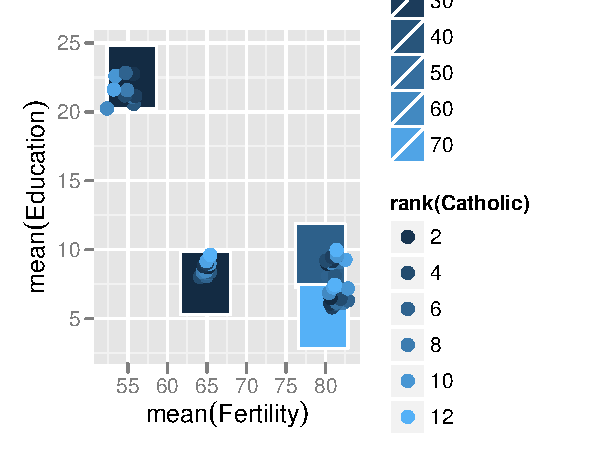
\includegraphics[width=0.49\textwidth]{figure/minimal-overlaps1} 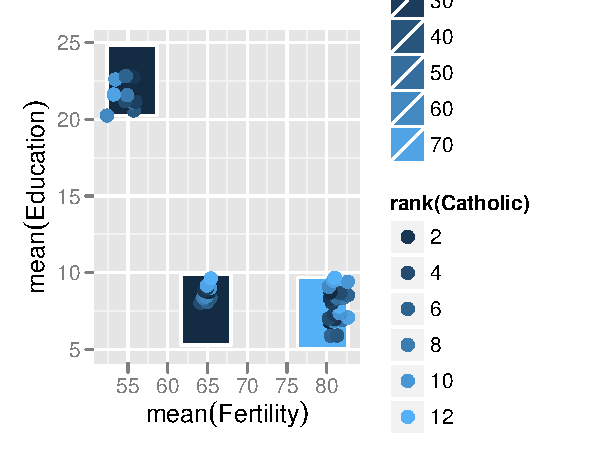
\includegraphics[width=0.49\textwidth]{figure/minimal-overlaps2} 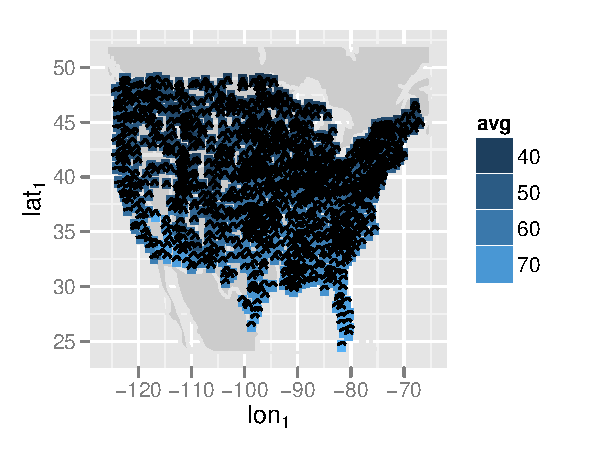
\includegraphics[width=0.49\textwidth]{figure/minimal-overlaps3} 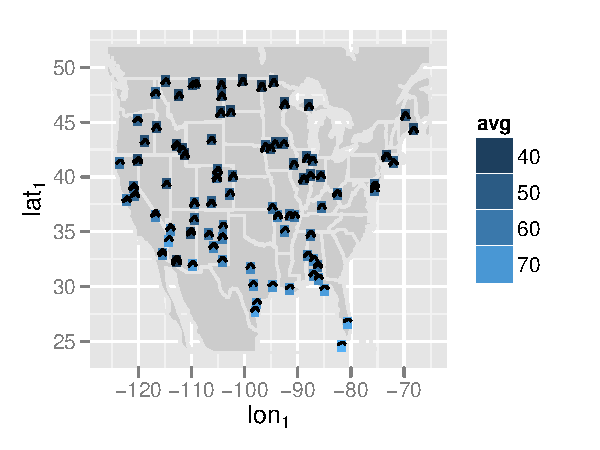
\includegraphics[width=0.49\textwidth]{figure/minimal-overlaps4} 

}


\end{knitrout}


\subsection{grid}
Gridding is the simplest way to embed subplots in a graph. \texttt{grid} basically bins a layer into a 2d grid of subplots and plots a glyph at every bin location. The syntax of \texttt{grid} is very similar to that of \texttt{glyph}. However, \texttt{grid} does not take \texttt{width}, \texttt{height}, or \texttt{merge.overlaps} arguments. the dimension of the glyphs (and the lack of overlaps) is implicit in the intention to grid a layer. Instead, \texttt{grid} takes two new arguments" \texttt{x.nbin} and \texttt{y.nbin}. These specify the number of bins to use on the x and y axiis. They are set to ten by default. 
Like \texttt{glyph}, \texttt{grid} can take reference and scale arguments.

\begin{knitrout}
\definecolor{shadecolor}{rgb}{0.969, 0.969, 0.969}\color{fgcolor}\begin{kframe}
\begin{flushleft}
\ttfamily\noindent
\hlcomment{\usebox{\hlnormalsizeboxhash}\usebox{\hlnormalsizeboxhash}{\ }without{\ }gridding}\hspace*{\fill}\\
\hlstd{}\hlfunctioncall{ggplot}\hlkeyword{(}\hlsymbol{test.data}\hlkeyword{)}{\ }\hlkeyword{+}{\ }\hlfunctioncall{geom\usebox{\hlnormalsizeboxunderscore}point}\hlkeyword{(}\hlfunctioncall{aes}\hlkeyword{(}\hlsymbol{Fertility}\hlkeyword{,}{\ }\hlsymbol{Education}\hlkeyword{)}\hlkeyword{)}\hspace*{\fill}\\
\hlstd{}\hlcomment{\usebox{\hlnormalsizeboxhash}\usebox{\hlnormalsizeboxhash}{\ }with{\ }gridding}\hspace*{\fill}\\
\hlstd{}\hlfunctioncall{ggplot}\hlkeyword{(}\hlsymbol{test.data}\hlkeyword{)}{\ }\hlkeyword{+}\hspace*{\fill}\\
\hlstd{}{\ }{\ }\hlfunctioncall{grid}\hlkeyword{(}\hlfunctioncall{geom\usebox{\hlnormalsizeboxunderscore}point}\hlkeyword{(}\hlfunctioncall{aes}\hlkeyword{(}\hlsymbol{Fertility}\hlkeyword{,}{\ }\hlsymbol{Education}\hlkeyword{)}\hlkeyword{)}\hlkeyword{,}{\ }\hlargument{x.nbin}{\ }\hlargument{=}{\ }\hlnumber{10}\hlkeyword{,}{\ }\hlargument{y.nbin}{\ }\hlargument{=}{\ }\hlnumber{10}\hlkeyword{,}\hspace*{\fill}\\
\hlstd{}{\ }{\ }{\ }{\ }{\ }{\ }{\ }\hlargument{ref}\hlargument{=}{\ }\hlfunctioncall{ref\usebox{\hlnormalsizeboxunderscore}box}\hlkeyword{(}\hlfunctioncall{aes}\hlkeyword{(}\hlargument{fill}{\ }\hlargument{=}{\ }\hlfunctioncall{mean}\hlkeyword{(}\hlsymbol{Catholic}\hlkeyword{)}\hlkeyword{)}\hlkeyword{)}\hlkeyword{)}\mbox{}
\normalfont
\end{flushleft}
\end{kframe}

{\centering 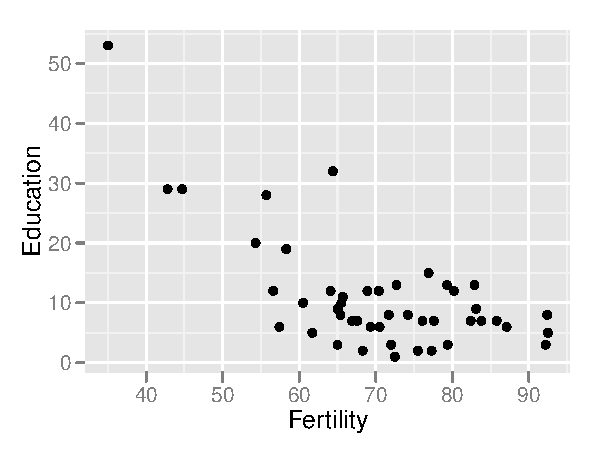
\includegraphics[width=0.49\textwidth]{figure/minimal-grids1} 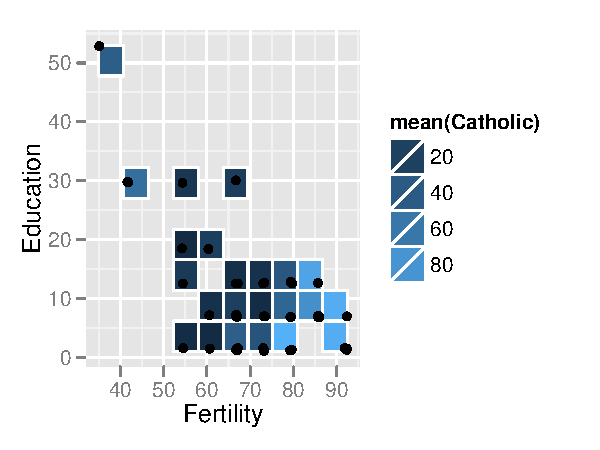
\includegraphics[width=0.49\textwidth]{figure/minimal-grids2} 

}


\end{knitrout}


Gridding provides a new way to approach the problem of overplotting. A grid of glyphs can work like a bin2d but provides more information. Figure~\ref{fig:overplotting} demonstrates this approach by recreating an overplotting graph that has garnered recent interest on the ggplot2 mailing list. 

\begin{knitrout}
\definecolor{shadecolor}{rgb}{0.969, 0.969, 0.969}\color{fgcolor}\begin{kframe}
\begin{flushleft}
\ttfamily\noindent
\hlcomment{\usebox{\hlnormalsizeboxhash}\usebox{\hlnormalsizeboxhash}{\ }without{\ }gridding}\hspace*{\fill}\\
\hlstd{}\hlsymbol{cheap.diamonds}{\ }\hlassignement{\usebox{\hlnormalsizeboxlessthan}-}{\ }\hlfunctioncall{subset}\hlkeyword{(}\hlsymbol{diamonds}\hlkeyword{,}{\ }\hlsymbol{price}{\ }\usebox{\hlnormalsizeboxlessthan}={\ }\hlnumber{5000}{\ }\hlkeyword{\usebox{\hlnormalsizeboxand}}{\ }\hlsymbol{price}{\ }\hlkeyword{\usebox{\hlnormalsizeboxgreaterthan}=}{\ }\hlnumber{600}\hlkeyword{)}\hspace*{\fill}\\
\hlstd{}\hlfunctioncall{ggplot}\hlkeyword{(}\hlsymbol{cheap.diamonds}\hlkeyword{)}{\ }\hlkeyword{+}\hspace*{\fill}\\
\hlstd{}{\ }{\ }\hlfunctioncall{grid}\hlkeyword{(}\hlfunctioncall{geom\usebox{\hlnormalsizeboxunderscore}bar}\hlkeyword{(}\hlfunctioncall{aes}\hlkeyword{(}\hlargument{x}{\ }\hlargument{=}{\ }\hlsymbol{color}\hlkeyword{,}{\ }\hlargument{fill}{\ }\hlargument{=}{\ }\hlsymbol{color}\hlkeyword{)}\hlkeyword{,}{\ }\hlargument{position}{\ }\hlargument{=}{\ }\hlstring{"{}dodge"{}}\hlkeyword{)}\hlkeyword{,}\hspace*{\fill}\\
\hlstd{}{\ }{\ }{\ }{\ }\hlargument{grid.aes}{\ }\hlargument{=}{\ }\hlfunctioncall{aes}\hlkeyword{(}\hlargument{x}{\ }\hlargument{=}{\ }\hlsymbol{carat}\hlkeyword{,}{\ }\hlargument{y}{\ }\hlargument{=}{\ }\hlsymbol{price}\hlkeyword{)}\hlkeyword{,}{\ }\hlargument{x.nbin}{\ }\hlargument{=}{\ }\hlnumber{10}\hlkeyword{,}{\ }\hlargument{y.nbin}{\ }\hlargument{=}{\ }\hlnumber{14}\hlkeyword{,}\hspace*{\fill}\\
\hlstd{}{\ }{\ }{\ }{\ }\hlargument{y\usebox{\hlnormalsizeboxunderscore}scale}{\ }\hlargument{=}{\ }\hlsymbol{free}\hlkeyword{,}{\ }\hlargument{height.adjust}{\ }\hlargument{=}{\ }\hlnumber{0.5}\hlkeyword{,}{\ }\hlargument{width.adjust}{\ }\hlargument{=}{\ }\hlnumber{0.5}\hlkeyword{,}\hspace*{\fill}\\
\hlstd{}{\ }{\ }{\ }{\ }\hlargument{ref}{\ }\hlargument{=}{\ }\hlfunctioncall{ref\usebox{\hlnormalsizeboxunderscore}box}\hlkeyword{(}\hlfunctioncall{aes}\hlkeyword{(}\hlargument{color}{\ }\hlargument{=}{\ }\hlfunctioncall{mean}\hlkeyword{(}\hlfunctioncall{as.numeric}\hlkeyword{(}\hlsymbol{color}\hlkeyword{)}\hlkeyword{)}\hlkeyword{)}\hlkeyword{)}\hlkeyword{)}\mbox{}
\normalfont
\end{flushleft}
\end{kframe}

{\centering 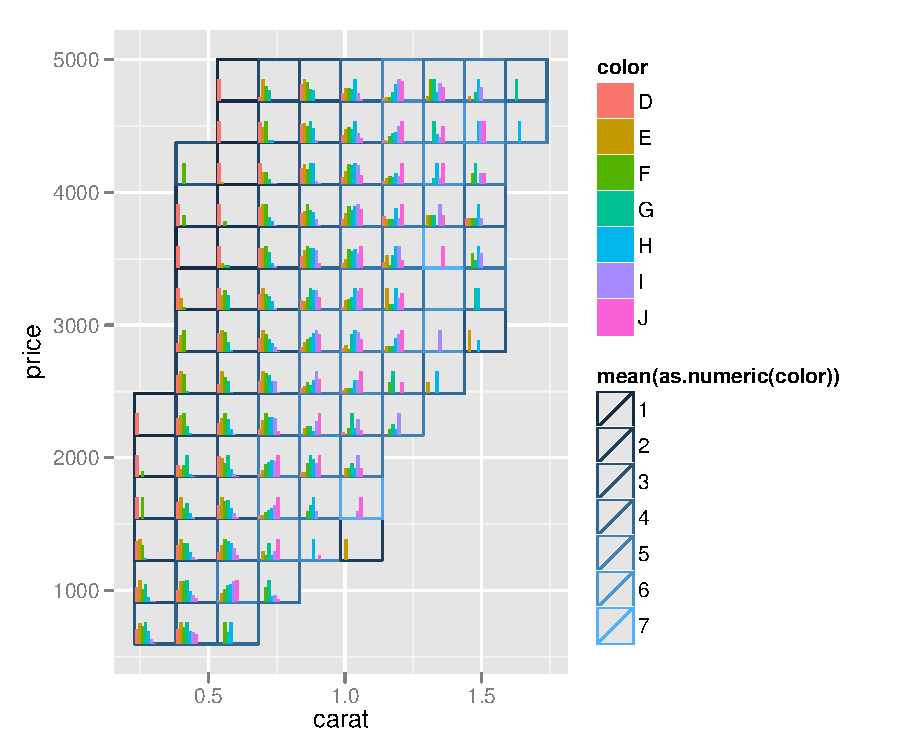
\includegraphics[width=\textwidth]{figure/minimal-overplotting} 

}


\end{knitrout}


\subsection{ply$\_$aes}







\bibliographystyle{plainnat}
\bibliography{ggplyr}
\end{document}
